% ================================================================== %
\documentclass{article}
\usepackage{mathsnotes}

% Course Details
\course{Graph Theory}
\term{Michaelmas 2024--25}
\lecturer{Stuart Martin}
\tripospart{Part II of the Mathematical Tripos}
\university{University of Cambridge}
\name{Avish Kumar}
\email{ak2461@cam.ac.uk}
\website{https://ak1089.github.io/maths/notes}
\version{2.0}
\disclaimer{These notes are unofficial and may contain errors. While they are written and published with permission, they are not endorsed by the lecturer or University.}

% Auxiliary files
\input{../graphs.tikzstyles}

% Format the document
\begin{document}
\makecover
% ================================================================== %

\section{Basics}
\subsection{Graphs}

Graph theory is really a subfield of combinatorics, an area of mathematics focused on problem-solving which comes up in a range of situations from machine learning to quantum field theory.

\begin{definition}[Graph]
	A \textit{graph} $G$ is an ordered pair of two sets:
	\begin{enumerate}
		\item the \textit{vertices} $V$ (also known as \textit{nodes}), and
		\item the \textit{edges} $E$, where the elements of $E$ are of the form $\set{\set{x, y} \mid x, y \in V \with x \neq y}$.
	\end{enumerate}
	In this course, we focus mainly on finite graphs: unless otherwise stated, $V$ and $E$ are finite.
\end{definition}

This definition lends itself to a canonical diagramattic representation for a graph. We draw the vertices as little circles, and draw a line representing each edge between the two points it connects.

\begin{example}[Basic Graphs]
	One type of basic graph is called a \textit{path}, written $P_n$ for the path of $n$ edges. This is given by $V = \set{1 \ldots n}$ and $E = \set{\set{1, 2}, \set{2, 3}, \ldots , \set{n-1, n} }$. For example, here is $P_5$:

	\ctikzfig{graph-example-p5}

	Another common graph is called a \textit{cycle}, written $C_n$ (for $n>2$). This is like a path, but it loops back around to the start (ie. $E$ also contains $\set{n, 1}$). Here is $C_6$:

	\ctikzfig{graph-example-c6}

	We also have $K_n$, the \textit{complete graph} on $n$ vertices, with every possible edge. Here is $K_4$:

	\ctikzfig{graph-example-k4}

	Lastly, we have $E_n$, the \textit{empty graph}, which has no edges. Here is $E_3$:

	\ctikzfig{graph-example-e3}

	There are, of course, more types of graph, but these are the most basic and most common.
\end{example}

\begin{note}
	We usually write $ab$ as shorthand for the edge $\set{a, b} \in E$.
\end{note}

\begin{note}
	There are some limitations inherent to this definition. The stipulation $x \neq y$ precludes loops (as a vertex cannot be connected to itself), $E$ being a set precludes multiple edges between a single pair of vertices, and the elements of $E$ being unordered precludes directed edges.
\end{note}

\begin{definition}[Order and Size]
    The \textit{order} of the graph $G = (V, E)$ is the number of vertices (that is, $\abs{G} = \abs{V}$). When we want the \textit{size} of the graph, which is the number of edges, we write $e(G) = \abs{E}$.
\end{definition}

In a lot of cases, these are easy to calculate. Thinking back to our four basic examples, we have
\begin{enumerate}
    \item $\abs{P_n} = n$ and  $e(P_n) = n-1$
    \item $\abs{C_n} = n$ and  $e(C_n) = n$
    \item $\abs{K_n} = n$ and  $e(K_n) = \frac{1}{2}n(n-1)$
    \item $\abs{E_n} = n$ and  $e(E_n) = 0$
\end{enumerate}

In general, when $xy$ is an edge, we say $x$ and $y$ are \textit{adjacent}, or \textit{neighbours}. More generally, the \textit{neighbourhood} of a vertex $x$ is the set $\Gamma (x)$ of vertices adjacent to it. The \textit{degree} of $x$ is the size of its neighbourhood. For example, every vertex in $K_n$ has degree $n-1$.

\begin{note}
	The degree sequence of a graph is then the list of degrees of its vertices. For example, $P_4$ has degree sequence 2, 2, 1, 1. The sum of the degree sequence of a graph must be an even number: specifically, twice the number of edges.
\end{note}

Now, let's look at isomorphisms between graphs. The basic idea is to regard graphs to be equivalent if they have the exact same structure. This gives us a natural definition:

\begin{definition}[Graph Isomorphism]
    Two graphs $G = (V, E)$ and $H = (V', E')$ are \textit{isomorphic} if there exists a bijection $f: V \to V'$ such that $xy \in E \iff f(x)f(y) \in E'$. $f$ is then a \textit{graph isomorphism}.
\end{definition}

We now look at subgraphs. We can generate subgraphs by optionally removing some vertices from $G$, removing all edges to and from those vertices, then removing some more edges if desired.

\begin{definition}[Subgraph]
    We say $H = (V', E')$ is a \textit{subgraph} of $G = (V, E)$, and write $H \leq G$, if
    \begin{enumerate}
        \item $V' \subs V$ and $E' \subs E$.
        \item $H$ is a graph in its own right.
    \end{enumerate}
\end{definition}

\begin{example}[Subgraph]
    A subgraph might look like:

    \ctikzfig{subgraph-definition}
\end{example}

When dealing with subgraphs, we often use the notation $G + xy$ to denote ``adding" the edge $x y$. Similarly, $G - x$ can be used to remove a vertex (and its edges).

\begin{definition}[Regularity]
	\label{regular-definition}
    A graph $G$ is $k$-\textit{regular} if every vertex has degree exactly $k$. Paths are generally not regular, but cycles are 2-regular.
\end{definition}

% ================================================================== %

\subsection{Connectedness}

We want to gain an understanding of how connected graphs are: in what ways can you travel between vertices along the edges of the graph? To do this, we look at \textit{paths}.

\begin{definition}[Path]
	\label{path}
    A \textit{path} in $G$ is a sequence of distinct vertices $x_1 \dots x_n$ such that $x_1 x_2$, $x_2 x_3$, and so on are all edges. If a path starts at $x_1 = x$ and ends at $x_n = y$, we call it an $x$-$y$ path of length $n$.
\end{definition}

 A graph is then called \textit{connected} if there is an $x$-$y$ path for every pair of vertices.

\begin{example}[Connectedness]
    The graph on the left is \textit{connected}, and the highlighted edges show a path between the vertices labelled $x$ and $y$. By contrast, the subgraph on the right is disconnected, due to the removal of a vertex and four edges: the equivalent $x'$ and $y'$ do not have a path between them.

    \ctikzfig{connections}
\end{example}

\begin{proposition}[Graph Connectedness]
	Define the relation $\sim$ on the vertices of a graph $G$ to mean $x \sim y$ if and only if there exists an $x$-$y$ path. Then $\sim$ is an equivalence relation.
\end{proposition}

\begin{prf}
	(Sketch) Of course, reflexivity and symmetry are obvious. Transitivity is actually \textit{not} obvious, since a simple concatenation might reuse edges (which is prohibited). However, the relation is indeed transitive, you can shorten the two paths until they meet at a unique point.
\end{prf}

The \textit{connected components} of a graph are the equivalence classes under $\sim$. The right graph in the last example would have two connected components, containing $x'$ and $y'$.

\begin{definition}[Walk]
	\label{walk-definition}
    A \textit{walk} is similar to a path, but listed in terms of the vertices and edges the path travels along rather than simply being a list of edges.
    
    Under our definition of graphs, where there is no self-adjacency and no repetition in a path, these two definitions are in fact equivalent.
\end{definition}

% ================================================================== %

\subsection{Trees}

We now consider a special type of graph, known as a tree.

\begin{definition}[Tree]
	A \textit{tree} is a connected graph which is \textit{acyclic} (doesn't contain any cycles). A \textit{leaf} is a vertex of a tree which has degree 1.

	\ctikzfig{tree-definition}
\end{definition}

\begin{proposition}[Properties of Trees]
	Let $G$ be a graph. Then the following are equivalent:
	\begin{enumerate}
		\item $G$ is a tree.
		\item $G$ is a maximal acyclic graph (adding any edge creates a cycle).
		\item $G$ is minimally connected (removing any edge disconnects $G$).
	\end{enumerate}
\end{proposition}

\begin{prf}
	($1 \Ra 2$) $G$ is acyclic and connected by definition. Take any $x$ and $y$ such that $xy$ is not an edge. But $G$ is connected, so there is an $x$-$y$ path. Thus adding the edge would create a cycle.

	($2 \Ra 1$) $G$ is acyclic by definition. If $x$ and $y$ are not connected, then $G + xy$ is a supergraph which is connected and still acyclic.

	($1 \Ra 3$) $G$ is connected by definition. Suppose $G - xy$ is still connected. Then there is an $x$-$y$ path $P$ such that $xy \notin P$. But then there must be a cycle $P+yx$, which is a contradiction.

	($3 \Ra 1$) $G$ is connected by definition. Suppose $G$ contains some cycle $C$. Choose an edge $xy \in C$, and consider $G - xy$. For vertices $a$ and $b$ of $G - xy$, consider a path $P$ connecting them: if $xy$ appears in this path, then replace it with the rest of $C$. Then $a$ and $b$ are still connected, so $G - xy$ is connected, contradicting minimality.
\end{prf}

\begin{proposition}[Existence of Leaves]
	Every tree with order at least 2 has a leaf.
\end{proposition}

\begin{prf}
	Suppose not. Then take a path of maximal length. Then take the end vertex of the path: it must be connected to another vertex which isn't just the previous vertex of the path, but then adding this vertex to the path either creates a cycle or extends the path, contradicting maximality. In fact, this proof shows that the graph must have at least \textit{two} leaves, as the same argument works for the start vertex. (In fact, $P_n$ has exactly two leaves.)
\end{prf}

\begin{proposition}[Size of Trees]
	Let $T$ be a tree of order $n$. Then $e(T) = n - 1$.
\end{proposition}

\begin{prf}
Given $G = (V, E)$, write $G(W)$ for the subgraph spanned by $W \subs V$, and $G - x$ for $G(V \setminus \set{x})$. We induct on $n$: the proposition is trivial for $n = 1$ and $n = 2$. If $T$ is a tree of order $n$, choose a leaf $x$ and consider $T - x$. This is acyclic, because we have removed a vertex and an edge (which cannot remove a cycle), and connected (no path between two other vertices can have used the single edge connected to $x$). Then $T - x$ is a tree with $n-1$ vertices, and so by the induction hypothesis has $n-2$ edges. So $T$ has one extra edge, ie. $n-1$ edges, as required.
\end{prf}

\begin{definition}[Spanning Tree]
	A \textit{spanning tree} on a graph $G$ is a subgraph of $G$ which is a tree and has all the same vertices.
\end{definition}

\begin{proposition}[Existence of Spanning Trees]
	Every connected graph has a spanning tree.
\end{proposition}

\begin{prf}
	A tree is a minimal connected graph. Take the connected graph and remove edges until it is minimal connected, and you are left with a tree.
\end{prf}

\begin{definition}[Distance]
	\label{distance-definition}
	For a graph $G = (V, E)$, the graph distance function $d$ is defined as
	\[
	d: V \times V \to \R_{\geq 0} \cup \set{\infty} : (x, y) \mapsto \begin{cases}
	\text{minimum $x$-$y$ path length if one exists} \\ \infty \otherwise
	\end{cases}
	\]
	In fact, this is a metric! The \textit{diameter} of $G$ is the maximum distance between two vertices.
\end{definition}

\begin{definition}[Forest, Bridge, Cutvertex]
	\label{forest-bridge-cutvertex}
	A \textit{forest} is an acyclic graph. As such, a forest is a graph $G$ in which every connected component of $G$ is a tree.
	  
	A \textit{bridge} is an edge $xy$ in a connected graph such that $G - xy$ is disconnected. Similarly, a \textit{cutvertex} is a vertex $x$ in a connected graph such that $G - x$ is disconnected.
\end{definition}

\begin{note}
	If $G$ has a bridge then it has a cutvertex, but the converse is not true. This is not obvious: for example not every vertex to which a bridge is indicent is a cutvertex, as it may have degree 1. However, using induction, this holds for trees, and using the fact that every graph has a spanning tree completes the proof.
\end{note}

% ================================================================== %

\subsection{Bipartite Graphs}

We now look at another special type of graph: bipartite graphs. As the name implies, these graphs have two distinct parts, and edges are between these parts rather than within them.

\begin{definition}[Bipartite Graph]
	\label{bipartite-definition}
	A graph $G$ is \textit{bipartite} if $V = V_1 \cup V_2$ such that $V_1 \cap V_2 = \emptyset$ and for all edges $xy \in E$, $x \in V_1 \iff y \in V_2$. These subsets are sometimes called the vertex classes.
\end{definition}

\begin{note}
	Later, we will meet the more general notion of an $r$-partite graph (Definition \ref{r-partite-graph}).
\end{note}

\begin{example}[Bipartite Graph]
    The following graph is bipartite, with $V_1$ and $V_2$ coloured differently.
    
    \ctikzfig{graph-cube}
    
    On the other hand, $C_5$ (or any odd cycle) is obviously not bipartite.

    The complete bipartite graph $K_{m,n}$ is the graph where $\abs{V_1} = m$, $\abs{V_2} = n$, and every possible edge is present. It has order $m + n$ and size $mn$. $K_{2,3}$ looks like this:
    
    \ctikzfig{graph-k23}
\end{example}

\begin{proposition}[Only even cycles are bipartite]
	For all $n$, the cycle $C_{2n}$ is bipartite but the cycle $C_{2n+1}$ is not.
\end{proposition}

\begin{prf}
	For any bipartite graph, we must have
	\[
	\sum_{v \in V_1} \deg v = \sum_{v \in V_2} \deg v = e(G)
	\]
	as each edge is counted exactly once in each vertex class.
	
	In a cycle, every vertex has degree 2, so we have $\abs{V_1} = \abs{V_2}$. This is obviously not possible for odd cycles, so these cannot be bipartite.
	
	In contrast, even cycles are clearly bipartite: choose alternating vertices as the vertex classes. All edges take the form $x_i x_{i+1}$ (or $x_{2n}x_1$), which means all edges are indeed between edges with opposite parity.
\end{prf}

\begin{definition}[Circuit]
    \label{circuit-definition}
    A circuit in $G$ is a closed walk (akin to a cycle, but with repeated vertices).
\end{definition}

\begin{proposition}[Bipartite Cycle Criterion]
	$G$ is bipartite if and only if it contains no odd cycles.
\end{proposition}

\begin{prf}
	 Any odd circuit contains an odd cycle. This can be shown by induction. First, it is true for $n = 3$. In general, if we have a circuit of distinct vertices, we are done. If not, there is a repeated vertex: say
	\[
	C = x_1 \ldots x_a z x_{a+2} \ldots x_b z x_{b+2} \ldots x_k
	\]
	Now, take the circuits 
	\[
	C_1 = x_1 \ldots x_a z x_{b+2} \ldots x_k \quad \text{and} \quad 
	C_2 = z x_{a+2} \ldots x_b z
	\]
	These have length less than that of $C$, and one of them must have odd length. By induction, there is an odd cycle, and so $C$ must have contained one too.
	
	If bipartite $G$ contains an odd cycle, there exists an odd cycle which is bipartite (clearly false).
	
	Now, we show that if $G$ has no odd cycles, then it is bipartite. Assume that it is connected: if not, we can simply apply this proof to a connected component of it.
	
	Fix $x_1 \in V$. Define $V_1$ to be the set $\set{x \in V : d(x, x_1) \text{ odd}}$, and $V_2 = V \setminus V_2$. This is a bipartition. If $x$ was adjacent to $y$, and $d(x, x_1) \equiv d(y, x_1) \mod 2$, then there would be an odd circuit $x_1 \ldots x y \ldots x_1$. Thus there would be an odd cycle, a contradiction.
\end{prf}

% ================================================================== %

\subsection{Planarity}

We now look at a property of graphs which has come to mind when drawing them on the page. It seems like some graphs are able to be drawn nicely on a page, with no lines crossing. However, others seem to always need lines crossing over each other: there is no way to embed them neatly into a plane. Let us formalise this intuition.

\begin{definition}[Planar Graph]
	A \textit{planar} graph is a graph which can be drawn on the plane with no pair of edges crossing. For example, $K_4$ is planar, despite the basic drawing containing a crossing in the centre.
	
	\ctikzfig{planar-graph-definition}
	
	The drawing on the right shows an embedding with no crossings.
\end{definition}

Paths and cycles are planar, but it's surprisingly difficult to find a general criterion!

\begin{definition}[Face]
    The \textit{faces} of a plane graph $G$ are the connected components of the plane $\R^2 \setminus G$ (that is, the entire plane except for the point vertices and line edges).
    
    The \textit{boundaries} of these faces are the edges to which they are adjacent.
\end{definition}

\begin{example}[Faces]
    The following graph drawing has four faces (note that the exterior is included).
    
    \ctikzfig{graph-face-boundary-definition}
    
    $F_1$ has a boundary given by a 4-cycle, as does $F_2$. $F_3$ has a boundary given by a 3-cycle, while $F_4$ (the exterior) is bounded by a 5-cycle.
    
    (Note that boundaries are not always cycles, especially in disconnected graphs.)
\end{example}

Unfortunately, the definitions of planar graphs, faces, and so forth have hitherto been somewhat vague. Let's formalise them.

First, we define a polygonal arc. For two points $x, y \in \R^2$, we say that a \textit{polygonal arc} from $x$ to $y$ is a finite union of closed straight-line segments $x_1x_2$, $x_2x_3$, and so on up to $x_{k-1}x_k$. We enforce $x = x_1$ and $x_k = y$, and that every segment is disjoint except for specific endpoints (ie. $x_2x_3$ intersects $x_3x_4$ at $x_3$ only).

Next, a \textit{drawing} of a graph $G$ where $V(G) = \set{v_1 \dots v_n}$ is defined by a set of distinct points $x_1 \dots x_n \in \R$, together with, for each edge $v_i v_j \in E$, a polygonal arc from $x_i$ to $x_j$. 

For two points $a$ and $b$ in $\R^2$, we say $a \sim b$ if there is a polygonal arc in $\R^2 \setminus G$ from $a$ to $b$. The equivalence classes of this connection relation are the connected components, or faces. The boundary of a face $F$ consists of $G$ intersected with the closure $\bar{F}$.

We assume the basic topology of $\R^2$. We know that the boundary of a face consists of vertices and line segments. It is then easy to show, for example, that a cycle has two faces, and that every tree is planar with exactly one face.

\begin{remark}[Similar Drawings $\neq$ Isomorphism]
    Drawings of isomorphic graphs can be genuinely different!
    
    \ctikzfig{drawings-of-isomorphic-graphs-different}
    
    The two graphs here are isomorphic, with the same points in the same places. Nevertheless, the left version has a face in the centre with a 6-cycle as its boundary, whereas the right version doesn't.
\end{remark}

\begin{theorem}[Euler's Formula]
    \label{eulers-formula}
    Let $G$ be a connected plane graph with $n > 0$ vertices, $e$ edges, and $f$ faces. Then
    \[
    n - e + f = 2
    \]
\end{theorem}

\begin{prf}
    The empty graph $E_1$ has one vertex, one face, and zero edges, so the formula holds.
    
    If $G$ contains a cycle $C$, then choose an edge $xy$ on $C$. Then $G' = G - xy$ is still connected, and the number of faces decreases by 1. Then the number of faces and edges have both decreased in tandem, and so the formula still holds.
    
    If $G$ contains no cycles, then it is a tree (since it is connected). Then $e = n - 1$, and $f = 1$, so the formula holds.
\end{prf}

\begin{corollary}
    Suppose $G$ is planar with $\abs{G} \geq 3$. Then $e \leq 3n - 6$.
\end{corollary}

\begin{prf}
    Without loss of generality, assume $G$ is connected. (If not, we can add edges to get a connected graph.)
    
    Draw $G$ in the plane with no edges crossing. Note that each face is bounded by at least three edges, and each edge is adjacent to exactly two faces. This gives us
    \[
    3f \leq \sum_{f \text{ a face}} \text{number of edges adjacent to } f \leq 2e
    \]
    and since $f = 2 - n + e$ by Euler's Formula (\ref{eulers-formula}), we have $e \leq 3n-6$ as required.
\end{prf}

\begin{corollary}
    $K_n$ is not planar for $n > 4$.
\end{corollary}

\begin{prf}
    $e(K_n) = n \cdot (n-1) \div 2 > 3n-6$ when $n > 4$.
\end{prf}

\begin{corollary}
    $K_{3,3}$ is not planar either.
\end{corollary}

\begin{prf}
    Bipartite graphs have no odd cycles, so each face is bounded by at least \textit{four} edges. This means the inequality obtained is stricter: in fact $4f \leq 2e$, and so $e \leq 2n - 4$, which does not hold for $K_{3,3}$ (where $e = 9$ and $n = 6$).
\end{prf}

\begin{definition}[Subdivision]
    A \textit{subdivision} of a graph $G$ is a graph $\hat{G}$ obtained by replacing some or all edges of $G$ with disjoint paths.
    
    \ctikzfig{subdivision-definition}
    
    The graph on the right is a subdivision of the graph on the left.
\end{definition}

\begin{proposition}[Subdivisions Preserve Planarity]
    A graph $G$ is planar if and only if any subdivision of it is planar.
\end{proposition}

\begin{prf}
    This is obvious by a drawing argument. To draw a subdivision of $G$ in a planar fashion, or to draw $G$ given a planar drawing of a subdivision of $G$, simply ignore the extra/missing vertices, and draw the polygonal arcs at the same points!
\end{prf}

Finally, we have the capstone theorem of this section: the necessary and sufficient condition for proving whether or not a graph is planar.

\begin{theorem}[Kuratowski's Theorem]
    \label{kuratowskis-theorem}
    A graph $G$ is planar if and only if it does not contain as a subgraph any graph isomorphic to a subdivision of $K_5$ or $K_{3,3}$.
\end{theorem}

\begin{prf}
    Omitted.
\end{prf}

This is our necessary and sufficient condition! To prove a graph is planar, just draw it. To prove a graph is non-planar, find a subgraph which is a subdivision of $K_5$ or $K_{3,3}$.

% ================================================================== %

\pagebreak
\section{Connectivity and Matchings}

\begin{definition}[Independence of Edges, Matching]
    Take a bipartite graph $G = (X \cup Y, E)$. Then a set of edges is \textit{independent} if none of its edges have any vertices in common.  A \textit{matching} from $X$ to $Y$ is consists of $\abs{X}$ independent edges. Alternatively, this is a set of edges $\set{xf(x)} \subs E$, where $f: X \to Y$ is injective.
\end{definition}

When does $G$ have a matching? We use what's known as ``mathmaker" terminology, which comes from a somewhat less progressive era, and names
\[
X = \set{\text{boys}} \quad \text{and} \quad Y = \set{\text{girls}}
\]
where we say there is an edge $xy$ if and only if Boy $x$ and Girl $y$ know each other. We want to ``marry" each boy to a girl he knows. This is impossible if:
\begin{enumerate}
	\item $\abs{X} > \abs{Y}$ (there are more boys than girls)
    \item there is a boy $x \in X$ with $\deg (x) = 0$ (who doesn't know anyone)
    \item if there are distinct boys $x_1, x_2 \in X$ with $\Gamma(x_1) = \Gamma(x_2) = \set{y}$ for some girl $y$ (if two boys only know the same one girl)
\end{enumerate}
Now suppose we have some subset of boys $A \subs X$. We write $\Gamma(A) = \bigcup_{x \in A} \Gamma(x)$. Of course, we require $\abs{\Gamma(A)} \geq \abs{A}$ for this subset to have a matching. Less obviously, this is the \textit{only} restriction!

\begin{theorem}[Hall's Marriage Theorem]
    \label{halls-marriage-theorem}
    Let $G = (X \cup Y, E)$ be a bipartite graph. Then $G$ has a matching from $X$ to $Y$ if and only if
    \[
	\abs{\Gamma(A)} \geq \abs{A} \quad \forall A \subs X.
	\]
\end{theorem}

\begin{prf}
    ($\Rightarrow$) Take some subset $A \subs X$. If the matching edges are $x_1y_1, x_2y_2, \dots$ then we certainly know $\set{y_1, y_2 \dots} \subs \Gamma(A)$, and so Hall's condition is met.
    
    ($\Leftarrow$) Noting that the $\abs{X} \leq 2$ cases are obvious, induct on the size of $X$.
    
    Suppose first that for all nonempty $A \subsetneq X$ such that $\abs{\Gamma (A)} > \abs{A}$. Then we can take $x \in X$ and $y \in \Gamma (x)$, and construct $G - x - y$. Note that this satisfies the criterion by inductive assumption.
    \[
	\abs{\Gamma_{G'}(A)} \geq \abs{\Gamma_G (A)} - 1 \geq \abs{A}
	\]
	We have a matching in $G'$ from $X \setminus \set{x}$ to $Y \setminus \set{y}$. Together with $xy$, which exists as $y \in \Gamma(x)$, we get a new matching.
	
	In the other case, we have some nonempty $A \subsetneq X$ with $\abs{\Gamma (A)} = \abs{A}$. Let $B = \Gamma(A)$, $G_1 = G[A \cup B]$ and $G_2 = G[(X \setminus A) \cup (X \setminus B)]$ (both bipartite).
	
	First, $G_1$ has a matching from $A$ to $B$. For $C \subs A$, we have $\abs{\Gamma_G (C)} = \abs{\Gamma_{G_1} (C)}\geq \abs{C}$.

	Next, $G_2$ has a matching from $(X \setminus A)$ to $(X \setminus B)$, by pretty much the same argument.
	
	Putting these two matchings together gives us a matching in $G$ from $X$ to $Y$.
\end{prf}

\begin{corollary}
    A matching of deficiency $d$ in a bipartite graph $G = (X \cup Y, E)$ contains $\abs{X} - d$ independent edges. $G$ has a matching of deficiency $d$ from $X$ to $Y$ if and only if every subset $A \subs X$ satisfies the condition $\abs{\Gamma(A)} \geq \abs{A} - d$.
\end{corollary}

\begin{prf}
    ($\Rightarrow$) Obvious.
    
    ($\Leftarrow$) Form $G'$ by adding $d$ new points to $Y$, each with neighbourhood $X$. There is then clearly a matching in $G'$, giving a matching of deficiency $d$ in $G$.
\end{prf}

\begin{note}
	In the boys and girls scenario, we add $d$ imaginary girls to $Y$, known to all boys. By the above theorem, we have a matching whereby at most $d$ boys are paired with imaginary girls (and so at least $\abs{X} \geq d$ are paired with real girls).
\end{note}

\begin{definition}[Transversal]
    Consider a family $S_1 \dots S_n$ of finite subsets of $\calX$. Then a \textit{system of distinct representatives} (SDR), or a \textit{transversal}, is a set of distinct $x_1 \dots x_n$ such that $x_i \in S_i$ for all $i$.
\end{definition}

\begin{corollary}
    The sets $S_1 \dots S_n$ have a transversal if and only if
    \[
	\abs{\bigcup_{i \in A} S_i} \geq \abs{A} \quad \forall A \subs \set{1, 2, \dots, n}
	\]
	Similarly, we say that there is a transversal of deficiency $d$ if we can replace $\abs{A}$ by $\abs{A} - d$.
\end{corollary}

\begin{note}
	This corollary is equivalent to Hall's Marriage Theorem (\ref{halls-marriage-theorem}), since a matching in a bipartite graph with vertex classes $X$ and $Y$ is a transversal of the neighbourhoods $\set{\Gamma(x): x \in X}$.
\end{note}

\begin{example}[Group Cosets]
    Let $G$ be a finite group with $H \leq G$ a subgroup of index $\abs{G : H} = n$. Take the left cosets and right cosets and represent them as
    \[
	L_1 \dots L_n = g_1 H \dots g_n H \qquad \text{and} \qquad R_1 \dots R_n = H g_1' \dots H g_n'
	\]
	Can we choose representatives of the $L_i$ whicha re also representatives of the $R_i$?
	
	We want to pick $g_1 \dots g_n$ such that $g_1 H \dots g_n$ are the left cosets and $H g_1 \dots H g_n$ are the right cosets (up to rearrangement). Equivalently, we need to pick a permutation $\pi$ of $\set{1 \dots n}$ such that $L_i \cap R_{\pi(i)} \neq \emptyset$ for all $i$.
	
	By Hall's Marriage Theorem, we need only show that $\abs{\Gamma(A)} \geq A$ for all $A \subs X$. But the size of the union of the $L_i$ is $\abs{A}\abs{H}$, so the union meets at least $\abs{A}$ right cosets (which are all of size $\abs{H}$). Therefore yes we can!
\end{example}

Now, we want to better quantify connectivity. For example, $C_n$ is connected, and removing any vertex leaves $P_{n-1}$, which is still connected. $P_n$ is also connected, but removing any non-endpoint vertex disconnects it.

Similarly, taking the cube graph, removing any two vertices does not disconnect the graph, but removing three can (by removing the three vertices adjacent to a reference vertex).

\begin{definition}[Connectivity]
    For a graph $G$ where $\abs{G} \geq 1$, the \textit{connectivity} $\kappa(G)$ is the size of the smallest set $S \subs V$ such that $G-S$ is either disconnected or a single point. If $\kappa(G) \geq k$, then we say $G$ is $k$-connected.
\end{definition}

\begin{example}[Connectivity]
    Any tree $T$ is 1-connected but not 2-connected.
    
    Cycles $C_n$ are 2-connected but not 3-connected.
    
    The cube is 3-connected.
    
    $K_n$ is $n-1$-connected.
\end{example}

% ================================================================== %

\subsection{Menger's Theorem}

It is sometimes the case that \textit{removing} a vertex makes the graph \textit{more} connected. For example, see the graph on the left below and its subgraph on the right.

\ctikzfig{connectivity-increasing-when-removing-vertex}

Here, the graph on the left is 1-connected but not 2-connected (removing the highlighted vertex would disconnect the graph). However, by removing the vertex labelled $x$ would create the graph on the right, which is in fact 3-connected.

The connectivity of a graph is at most the ``minimum degree" $\delta(G) = \inf \set{\deg(x): x \in V}$. This is because one can choose the neighbourhood of some $x$ with that degree, and remove all the vertices in said neighbourhood.

In the same way that $G$ being connected means there is an $a$-$b$ path for every vertex pair in $G$, it would be nice if $G$ being $k$-connected means that there are $k$ such independent paths. (Here, two paths are independent if their intersection is just $\set{a, b}$).

\begin{definition}[Separator]
    Given distinct vertices $a$ and $b$ in a graph $G$, we say that the set $S \subs V(G) \setminus \set{a, b}$ \textit{separates} $a$ and $b$ if they are in different connected components of $G - S$, or equivalently if every $a$-$b$ path intersects $S$ somewhere.
    
    \ctikzfig{separator-definition}
    
    In this graph, the highlighted vertices form a \textit{separator}. When you remove them to get the graph on the right, $a$ and $b$ no longer have a path between them.
\end{definition}

This brings us to a significant result.

\begin{theorem}[Menger's Theorem]
    \label{mengers-theorem}
    For a graph $G = (V, E)$, let $a$ and $b$ be distinct non-adjacent vertices. Then if every separator $S \subs V$ of $a$ and $b$ has size at least $k$, then there is a family of $k$ independent $a$-$b$ paths.
\end{theorem}

\begin{remark}[Notes on Menger's Theorem]
    Before we prove this theorem, we first note a few things.
	\begin{enumerate}
	    \item The converse is trivial: any separator contains at least one point from each of $k$ paths.
	    \item It is equivalent to state that the minimum size of any $a$-$b$ separator is the maximum number of independent paths. (This is similar to the ``max-flow-min-cut" theorem).
	    \item The non-adjacency criterion is needed to allow the existence of a separator at all. If $x$ and $y$ are adjacent, in fact no set separates them, since the path $xy$ of length 2 exists.
	    \item In fact,  this is a generalisation of Hall's Marriage Theorem (\ref{halls-marriage-theorem}).
	\end{enumerate}
\end{remark}

Given bipartite $G = X \cup Y$ satisfying the Hall criterion, form $G'$ by adding vertices $s$ and $t$ joined to all of $X$ and $Y$ respectively.

Then $G$ has a matching if and only if $G'$ has a family of $\abs{X}$ independent $s$-$t$ paths, so it is enough to check that every separator has size at least $\abs{X}$. Take a separator $S$ with $A = S \cap X$ and $B = S \cap Y$. Then $\Gamma(X \setminus A) \subs B$, so $\abs{S} = \abs{A} + \abs{B} \geq \abs{\Gamma(X \setminus A)} + \abs{A} \geq \abs{X \setminus A} + \abs{A} = \abs{X}$.

Now, let's get to the actual proof of the theorem!
    
\begin{prf}
    Noting that the $k = 1$ case is clear, assume $k \geq 2$. Now, $k$ is the minimum size of an $a$-$b$ separator, and we seek $k$ independent paths from $a$ to $b$.
    
    Suppose, by way of contradiction, that this is not possible. Choose a minimal counterexample, with a smallest working $k$ and the minimum edges for that $k$. Let $S$ be a separator of that size.
    
    Suppose first that there is a separator $S \neq \Gamma(a)$ with $S \neq \Gamma(b)$. Form the graph $G'$ from $G$ by replacing the component of $G-S$ containing $a$ by a single point $a'$ adjoined to all of $S$. Then $e(G') < e(G)$, otherwise $\Gamma(a) \subs S$ and hence $\Gamma(a) = S$.
    
    In $G'$, there is no separator of size less than $k$, otherwise this set would also separate $a$ and $b$ in $G$. So by minimality, there exist $k$ paths in $G'$. This gives you $k$ paths $P_1 \dots P_k$ from $b$ to $S$ disjoint except at $b$. Similarly, we have $Q_1 \dots Q_k$ from $a$ to $S$ disjoint except at $a$.
    
    No $P_i$ and $Q_j$ can meet except at $S$, so we can join them to make $k$ independent paths in $G$.
    
    Suppose that every $a$-$b$ separator of size $k$ is equal to either $\Gamma(A)$ or $\Gamma(b)$. Observe that these two neighbourhoods are disjoint, otherwise take $x \in \Gamma(b) \cap \Gamma(a)$ and consider $G' = G - x$. All separators in $G'$ have size at least $k-1$, as with $x$ they separate $a$ and $b$ in $G$. By minimality of $k$, there are $k-1$ independent paths in $G'$. Then you can add $axb$ as another path to make $k$ independent paths in $G$.
    
    Now consider a shortest path from $a$ to $b$: $a x_1 x_2 \dots x_r b$. Take $G' = G - x_1 x_2$. Then $G'$ has a separator $S \neq \emptyset$ of size $k-1$. Consider $S \cup \set{x_1}$ and $S \cup \set{x_2}$: these are separators in $G$ of size $k$.
    
    As $x_1 \notin \Gamma(b)$, $S \cup \set{x_1} \neq \Gamma(b)$. Similarly, $S \cup \set{x_2} \neq \Gamma(a)$. Then $S \cup \set{x_1} = \Gamma(a)$ and $S \cup \set{x_2} = \Gamma(b)$. But then the intersection $\Gamma(a) \cap \Gamma(b) \neq \emptyset$, a contradiction.
\end{prf}

\begin{corollary}
    Let $G$ be a graph with more than one vertex. Then $G$ is $k$-connected if and only if there are $k$ independent paths between any pair of vertices $a$ and $b$. (``Vertex Menger")
\end{corollary}

\begin{prf}
    ($\Leftarrow$) $G$ is certainly connected with more than $k$ vertices. Also, for sets $S \subs V$ with $\abs{S} < k$, $G-S$ is connected, otherwise choose $a$ and $b$ in different components.
    
    ($\Rightarrow$) If $a$ and $b$ are non-adjacent, just apply Menger's Theorem (\ref{mengers-theorem}). If they \textit{are} adjacent, then $G' = G - ab$ must have $k-1$ independent paths. Then add the path $ab$ to get all $k$.
\end{prf}

\begin{definition}[Edge Connectivity]
    For a connected graph $G$, define the \textit{edge connectivity} of $G$ to be
    \[
	\lambda(G) = \inf \set{\abs{S}: S \subs E(G), G-S \text{ disconnected}}
	\]
	Then $G$ is $k$-edge connected if and only if $\lambda(G) \geq k$.
\end{definition}

\begin{note}
	This is not the same as connectivity! The graph on the left is 1-connected (with cutvertex in blue) but 2-edge connected (no bridge). The converse is impossible (see the note after \ref{forest-bridge-cutvertex}).
\end{note}
	
\ctikzfig{edge-connectivity-definition-cutvertex}

\begin{definition}[Edge-Disjoint]
    If paths $P_1 \dots P_k$ from $a$ to $b$ have pairwise disjoint edges, then we say they are \textit{edge-disjoint}. This is a different condition to independence:
    \ctikzfig{edge-disjoint-vs-independent}
    
    The two highlighted $a$-$b$ paths have a common vertex, so they are not independent. However, they do not share any edges, so they are edge-disjoint.
\end{definition}

\begin{definition}[Line Graph]
    \label{line-graph-definition}
    The \textit{line graph} $L(G)$ is the dual version of a graph $G$. The vertex set $V_L$ is the edge set $E_G$, and two vertices in $V_L$ are adjacent if they share a vertex in $G$.
    \ctikzfig{line-graph-definition}
    
    For example, the graph on the left has 8 edges. Each maps to a vertex in the line graph on the right, with adjacencies if and only if two edges meet n $G$.
\end{definition}

\begin{corollary}
	Let $G = (V, E)$ be a graph with distinct $a \neq b \in V$. Then the minimum size of the set $S \subs E$ separating $a$ and $b$ is the number of edge-disjoint $a$-$b$ paths. (``Edge Menger")
\end{corollary}

\begin{prf}
	Form $G'$ from $L(G)$ by adding $a'$ adjacent to every $e \in E_G$ incident with $a \in G$, and $b'$ similarly. If there is a family of independent $a$-$b$ paths in $G$, there is an equivalent family of $a'$-$b'$ graphs in $G'$. Apply the previous corollary to $G'$: these are precisely the $k$ edge-independent paths we are looking for.
\end{prf}

\begin{corollary}
    Let $G$ be a graph with $\abs{G} > 1$. Then $G$ is $k$-edge connected if and only if there are $k$ edge-disjoint $a$-$b$ paths for every pair of distinct vertices $a \neq b$.
\end{corollary}

\begin{prf}
    Obvious by previous corollaries.
\end{prf}

% ================================================================== %

\pagebreak
\section{Extremal Graph Theory}

This section looks at graphs which satisfy some sort of maximal property.

\begin{definition}[Eulerian Circuit]
    An \textit{Eulerian circuit} is a circuit (\ref{circuit-definition}) which passes through each edge of a graph exactly once. A graph $G$ which admits an Eulerian circuit is called \textit{Eulerian}.
\end{definition}

\begin{example}[Eulerian Graphs]
    \label{eulerian}
    The below graph is Eulerian: follow the numbered arrows to start and finish at the vertex labelled $x$, passing through all nine edges.
    
    \ctikzfig{eulerian-graph-example}
    
    Any graph with a bridge cannot be Eulerian, but the converse of this is false. (Unrelatedly, the famous K{\" o}nigsberg graph, which has seven bridges of a different kind, is not Eulerian.)
\end{example}

\begin{theorem}[Euler's Theorem]
    A connected graph is Eulerian if and only if every vertex has even degree.
\end{theorem}

\begin{prf}
    ($\Rightarrow$) If an Eulerian circuit passes though a vertex $x$ a total of $k$ times, then $d(x) = 2k$.
    
    ($\Leftarrow$) Suppose $G$ is a minimal counterexample (fewest edges). That is: we have a connected graph $G$ with $e(G) > 0$ and $d(x)$ even for all $x$, with $G$ not Eulerian.
    
    Let $C$ be the longest circuit in $G$ with no edges repeated. Note such a cycle exists: no vertex has degree 1, so $G$ cannot be a tree. Since $G$ is not Eulerian, $e(C) \neq e(G)$. Let $H$ be a component of $G - E(C)$ with $e(H) > 0$: one must exist, as not all edges of $G$ are in $C$.
    
    Now, every vertex in $H$ has even degree, so $H$ has an Eulerian circuit $C'$ by minimality. But then we can combine $C$ and $C'$, since they are disjoint and meet at a vertex (as $G$ is connected) to get a longer circuit with no repeated edge, which contradicts $C$ being the largest circuit.
\end{prf}

\begin{definition}[Hamiltonian Graph]
    A \textit{Hamilton Cycle} in a graph $G$ is a cycle which visits each vertex exactly once. A connected graph with such a cycle is called \textit{Hamiltonian}.
\end{definition}

Much like previous questions like the subgraph problem, we might wonder if there exists a nice necessary and sufficient condition for a graph to contain such a Hamiltonian cycle. Unfortunately, there is not. The problem of finding one is in fact a special case of the famous Travelling Salesman Problem, and is therefore NP-complete.

\begin{definition}[Complement]
    For a graph $G$, we can define the complement graph $\bar{G}$ as the graph with the same vertices but the opposite edges: $a$ and $b$ are adjacent in $G'$ if and only if they are not adjacent in $G$.
\end{definition}

\begin{note}
	Clearly, any vertex $x$ with degree 1 prevents $G$ from being Hamiltonian.
\end{note}

Recall the \textit{minimum degree} $\delta(G) = \inf \set{d(x): x \in V}$ of a graph $G$.

Is there a value of $\delta(G)$ which ensures $G$ is Hamiltonian?

\begin{theorem}[Dirac's Theorem on Hamiltonian Cycles]
    \label{diracs-theorem-on-hamiltonian-cycles}
    Every graph $G$ of order $n \geq 3$ with $\delta(G) \geq n/2$ is Hamiltonian.
\end{theorem}

\begin{prf}
    Assume $G$ is a counterexample. Note that $G$ is connected. Suppose $x$ and $y$ are not adjacent. We know that $\Gamma(x), \Gamma(Y) \subs V \setminus \set{x, y}$ and that $\abs{\Gamma(x)}, \abs{\Gamma(x)} \geq n/2$. This means that the intersection of the two neighburhoods is non-empty, by the pigeonhole principle.
    
    Let $P = x_1 x_2 \dots x_l$ be the longest path in $G$, so $l \geq 3$. Note that $G$ does not have an $l$-cycle: if $l = n$ then we're done, otherwise as $G$ is connected there is a vertex $x$ connected to the cycle from outside it, giving a path on $l+1$ points. Then $x_lx_1 \notin E$.
    
	Suppose we have a $1 \leq i < l$ such that there is an $x_i$-$x_l$ path and an $x_{i+1}-x_1$ path. This would form the cycle $x_1 \dots x_i x_l x_{l-1} \dots x_{i+1} x_1$.
	
	Define $\Gamma^+ (x_l) = \set{x_i: x_{i-1} \in \Gamma(x_l), 2 \leq i \leq l}$. Then this definitely does not intersect $\Gamma(x_1)$, by construction. However, the size of each of these is at least $n/2$, and they are both subsets of the maximal path $\set{x_2 \dots x_l}$.
\end{prf}

\begin{proposition}[Path Subgraphs]
    \label{must-contain-path-subgraph}
    Let $G$ be a connected graph of order $n \geq 3$, with $\delta(G) \geq k/2$ for some integer $k < n$. Then $P_k \leq G$: $G$ contains a path of length $k$.
\end{proposition}

\begin{prf}
    Suppose not. Then let $P = x_0 x_1 \dots x_l$ be a path of maximal length, for some $l < k$. The neighbours of $x_0$ and $x_l$ must be inside $P$, due to maximality. Let
    \[
	A = \Gamma(x_1) \qquad B = \set{x_{i+1} : x_i \in \Gamma(x_l)}
	\]
	These sets each have size at least $\delta(G) \geq k/2$. Also, $x_0$ is not in either set, so they are both subsets of $\set{x_1 \dots x_l}$, which is of size at most $l < k$. Their intersection is thus non-empty.
	
	Now, take $x_i \in A \cap B$, and consider the cycle $C$ of length $l$:
	\[
	C = x_0 x_i x_{i+1} x_{i+2} \dots x_{l-1} x_l x_{i-1} x_{i-2} \dots x_2 x_1 x_0 
	\]
	Since $l < n$, there is at least one vertex $c \notin C$, and since $G$ is connected, there is a path from $c$ to some vertex $x_j \in C$. Combining these, we can construct a path with length at least $l + 1$. This contradicts maximality, so we are done.
\end{prf}

\begin{theorem}[Edge Condition on Path Subgraphs]
    \label{edge-condition-on-maximal-path-subgraph}
    Let $G$ be a graph on $n \geq 3$ points. Then for $k \geq 1$,
    \[
	e(G) > \frac{n(k-1)}{2} \implies P_k \leq G.
	\]
\end{theorem}

\begin{prf}
    Assume $k \geq 2$, noting that the $k=1$ case is obvious, and induct on $n$. Also, if $n \leq k$, this is trivially true, as the condition is impossible to satisfy.
    
    Without loss of generality, take $G$ to be connected: if not, we can apply the proof to its connected components.
    
    By Proposition \ref{must-contain-path-subgraph}, we have a vertex $x$ of degree at most $(k-1)/2$. Let $G' = G - x$ be a graph on $n-1$ vertices, which by induction does not contain a path of length $k$. Thus
    \[
	e(G) = e(G') + d(x) \leq \frac{(n-1)(k-1)}{2} + \frac{k-1}{2} \leq \frac{n(k-1)}{2}
	\]
\end{prf}

% ================================================================== %

\subsection{Tur\'an's Theorem}

We often ask how ``large" (in some relevant sense) a graph with some given property can be. These are extremal problems: the last few we have seem have been about both cycles and paths. What about complete subgraphs?

\begin{definition}[$r$-partite Graphs]
	\label{r-partite-graph}
    We say that a graph $G$ is $r$-partite if there is a partition $V = V_1 \cup \dots \cup V_r$ of pairwise disjoint sets of vertices such that for all edges $xy \in E$, $x$ and $y$ are not in the same $V_i$.
    
    In the case where $r=2$, this is exactly a bipartite graph (Definition \ref{bipartite-definition}).
\end{definition}

\begin{definition}[Tur\'an Graph]
    The \textit{complete} $r$-partite graph has every edge between vertices in different classes of the partition: any edge being added to it makes it no longer $r$-partite.
    
    The Tur\'an graph $T_r(n)$ is the complete $r$-partite graph on $n$ vertices, with the size of the vertex classes ``as equal as possible" (differing by at most 1).
\end{definition}

\begin{remark}[Notes on Tur\'an graphs]
    There are some points to note from these definitions.
	\begin{enumerate}
	    \item If $G$ is $(r-1)$-partite, then $G$ does not contain $K_r$, otherwise two vertices of $K_r$ would be in the same class.
	    \item $T_{r-1}(n)$ therefore does not contain $K_r$.
	    \item If $r \divides n$, then all classes have size exactly $n/r$. This means the degree of every vertex is $n - n/r$, or alternatively $n(1-1/r)$.
	    \item To obtain $T_r(n-1)$ from $T_r(n)$, you can remove any point from any largest class.
	    \item To do the opposite, add a point to any smallest class, and all possible edges.
	\end{enumerate}
\end{remark}



\begin{theorem}[Tur\'an's Theorem]
    \label{turans-theorem}
    Let $G$ be a graph on $n$ vertices. Then if $e(G) > e(T_{r-1}(n))$, then $K_r \leq G$.
\end{theorem}

\begin{note}
	This is the best possible bound: the Tur\'an graph is maximal. However, generally $e(T_{r-1}(n))$ is a fairly complicated function of both $n$ and $r$.
\end{note}

\begin{prf}
    By maximality, it is sufficient to show that
    \[
	\abs{G} = n, e(G) = e(T_{r-1}(n)), K_r \not\leq G \implies G \cong T_{r-1}(n).
	\]
	Induct on $n$, assuming $n \geq r$ (the other cases are clear). Notice that $\delta(G) \leq \delta(T_{r-1}(n))$.
	
	We claim that for any vertex $x \in G$ with $d(x) = \delta(G)$, $G' = G - x = T_{r-1}(n-1)$. Note that that $G'$ does not contain $K_r$, and has $e(G) - \delta(G)$ edges, which is at least $e(T_{r-1}(n)) - \delta(T_{r-1}(n))$. This last expression is the same as $e(T_{r-1}(n-1))$, by point 4 above. By induction, $G'$ is indeed the Tur\'an graph on one fewer vertex.
	
	Now, let $V_1 \dots V_{r-1}$ be vertex classes of $G'$. But $\Gamma(x)$ must miss some $V_i$, otherwise $G \geq K_r$. Then $\Gamma(x) \cap V_i \neq \emptyset$ for some $i$. But $\abs{\Gamma(x)} = n-1 - \min \abs{V_i}$. So
	\[
	\Gamma(x) = \bigcup_{j \neq i} V_j \qquad \abs{V_i} \text{ minimal}
	\]
	$G$ is then complete $(r-1)$-partite with vertex classes $V_j (j \neq i)$ and $V_i \cup \set{x}$, so $G \cong T_{r-1}(n)$.
\end{prf}

\begin{example}[The Problem of Zarankiewicz]
    \label{problem-of-zarankiewicz-example}
    How many edges can a bipartite graph with $n$ vertices per class have without containing $K_{t,t}$? We write $Z(n, t)$ for this size. Traditionally, we think of $t$ as being fixed, amd varying $n$ and looking at asymptotic behaviour.
\end{example}

\begin{theorem}[The Problem of Zarankiewicz]
    \label{problem-of-zarankiewicz-theorem}
    Let $t \geq 2$. Then $Z(n, t)$ is subquadratic: indeed $Z(n, t) \leq 2n^{2-1/t}$ for sufficiently large $n$.
\end{theorem}

\begin{prf}
    Recall that we need $G = (X \cup Y, E)$ with $\abs{X} = \abs{Y} = n$, where $G \not\geq K_{t,t}$. Let the degrees in $X$ be $d_1 \dots d_n$. We can freely take $d_i \geq t-1$ (if not, just add them in for extra edges).
    
    For each $t$-set $S \subs Y$, count how many $x \in X$ have $S \subs \Gamma(x)$. Of course, this must be at most $t-1$. Thus the number of
    \[
	(x, S) \in X \times \set{\abs{S} = t: S \in \powerset{Y}} \suchthat S \subs \Gamma(x) \quad \leq \quad (t-1) {n \choose t}
	\]
	Now, each $x$ belongs to exactly $d(x)$ choose $t$ such pairs. Thus
	\[
	\sum_{x \in X} d(x) = \sum_{i = 1}^n d_i \leq (t-1) {n \choose t}
	\]
	Now consider that the function
	\[
	w \mapsto w \times (w - 1) \times \dots \times (w - t + 1) \div t!
	\]
	is convex in $w$ for $w \geq t-1$. This means that
	\[
	\sum {d_i \choose t} \geq n {d \choose t} \quad \where d = \frac{1}{n} \sum d_i
	\]
	\[
	\implies n(d- t + 1)^t \leq (t-1) n^t \implies d \leq (t-1)^{1/t} n^{1-1/t} + t - 1
	\]
	\[
	\implies nd = e(G) \leq t^{1/t} \cdot n^{2-1/t} + tn
	\]
	which gets us the required result.
\end{prf}

But does $Z(n, t)$ actually grow at that rate? Well, this is an unsolved problem! For sufficiently large $n$, $Z(n, 2)$ can be bounded between $C_1 n^{3/2}$ and $2 n^{3/2}$, while $Z(n, 3)$ can be bounded between $C_2 n^{5/3}$ and $2 n^{5/3}$ (for some values of the constants $C_1$ and $C_2$).

\begin{definition}[Extremal Function]
    Take a fixed graph $H$. Define the \textit{extremal function} $\mathrm{ex}(n, H)$ to be the largest graph on $n$ vertices which does not contain a copy of $H$:
    \[
	\mathrm{ex}(n, H) = \max \set{e(G): \abs{G} = n, H \not\leq G}
	\]
\end{definition}

We can rewrite Tur\'an's theorem (\ref{turans-theorem}) to say
\[
\lim_{n \to \infty} \frac{2 \cdot \mathrm{ex}(n, K_r)}{n(n-1)} = 1 - \frac{1}{r-1}
\]
and Theorem \ref{edge-condition-on-maximal-path-subgraph} to say that $\mathrm{ex}(n, P_k) \sim n(k-1)/2$. We often refer to the limiting term as being the \textit{density} of the graph, since it is the proportion of possible edges which exist.

In general, how does this function $\mathrm{ex}(n, H)$ behave? Given $H$, let $r$ be the least integer such that $H$ is $r$-partite. Trivially, this is at most $\abs{H}$. Now consider $K_r(t)$, the complete $r$-partite graph with $t$ vertices per class, known as the ``$t$-blowup of $K_r$". 

\begin{theorem}[Erd{\H o}s-Stone Theorem]
    \label{erdos-stone-theorem}
    For all integers $r \geq 2$ and $t \geq 1$, and any $\eps > 0$, there is an integer $N$ such that if $G$ is a graph with $\abs{G} = n > N$,
    \[
	\mathrm{density}(G) = \frac{2 \cdot e(G)}{n(n-1)} > 1 + \frac{1}{r-1} + \eps \implies G \geq K_r(T)
	\]
\end{theorem}

\begin{prf}
    Omitted.
\end{prf}

\begin{corollary}
    \[
	\lim_{n \to \infty} \frac{2 \cdot \mathrm{ex}(n, H)}{n(n-1)} = 1 - \frac{1}{r-1} \qquad \with H \, r\text{-partite}
	\]
\end{corollary}

\begin{prf}
    Combine the reformulation of Turan's theorem and the fact that $H \leq K_r(t)$ for some $t$.
\end{prf}

\begin{note}
	If $H$ is bipartite specifically, then this is equal to 0: the graph is sparse. But the growth of $\mathrm{ex}(n, H)$ is generally mysterious, even for small $n$. For example, when $H = C_{2k}$, we only have any understanding of the cases up to $k = 5$.
\end{note}

% ================================================================== %

\pagebreak
\section{Graph Colouring}
\subsection{The Chromatic Number}

A graph colouring is a way of assigning each vertex of a graph a colour, such that no two adjacent vertices share a colour. For example, the graph below can be coloured using red, green, and yellow.

\ctikzfig{graph-colouring-3-colours}

\begin{definition}[$r$-colouring and Chromatic Number]
    \label{r-colouring-definition}
    An $r$-colouring of $G = (V, E)$ is a function $c: V \to \set{1 \dots r}$ with no adjacent edges mapping to the same colour, ie. $xy \in E \implies c(x) \neq c(y)$.
    
    The \textit{chromatic number} $\chi(G)$ is the smallest $r$ such that $G$ has an $r$-colouring. For example, the above graph has a chromatic number of 3 (the triangle ensures it cannot be 2-coloured).
\end{definition}

Obviously, $\chi(P_n) = 2 (n \geq 2)$, $\chi(E_n) = 1$, $\chi(K_n) = n$, and
\[
\chi(C_n) = \begin{cases}
	2 & n \text{ even} \\
	3 & n \text{ odd}
\end{cases}.
\]
\begin{note}
	In fact, for all trees, $\chi(T) = 2$: this is easy to show by induction, removing leaves.
\end{note}

\begin{proposition}[Bipartite is 2-Colourable]
    $G$ is bipartite is and only if $\chi(G) \leq 2$.
\end{proposition}

\begin{prf}
    ($\Rightarrow$) If $V = X \cup Y$, then set $c(x) = 1$ for $x \in X$ and $c(y) = 2$ for $y \in Y$. There are no edges between two vertices in $X$ or two vertices in $Y$, so the colouring rule holds.
    
    ($\Leftarrow$) Take $X = \set{x \in G: c(x) = 1}$ and $Y = \set{y \in G: c(y) = 2}$.
\end{prf}

\begin{note}
	In fact, in general $G$ is $r$-partite if and only if $\chi(G) \leq r$. This is the interpretation of the chromatic number: $\chi(G)$ is the least $r$ such that $G$ is $r$-partite. 
\end{note}

\begin{corollary}
    All trees are bipartite.
\end{corollary}

\begin{corollary}
    We can restate the Erd{\H o}s-Stone Theorem (\ref{erdos-stone-theorem}) in terms of the chromatic number:
	\[
	\lim_{n \to \infty} \frac{2 \cdot \mathrm{ex}(n, H)}{n(n-1)} = 1 - \frac{1}{\chi(H)-1}
	\]
\end{corollary}

What can we say about this chromatic number? For example, we can say that $\chi(G) \leq \abs G$: if we give each vertex a unique colour, then obviously the colouring is valid.

\begin{proposition}[Maximum Chromatic Number]
    \label{bound-on-chi}
    For any graph $G$, $\chi(G) \leq \Delta(G) + 1$, where $\Delta(G) = \max \set{d(x) : x \in G}$.
\end{proposition}

Before we prove this proposition, we should define an algorithm for colouring.

\begin{definition}[Greedy Colouring Algorithm]
    Given $G = (V, E)$ where $V = \set{v_1 \dots v_n}$, the \textit{greedy colouring algorithm} of $G$ on an ordering $v_1 \dots v_n$ is the process of:
    \begin{enumerate}
    \item Give $v_1$ colour 1.
    \item Give $v_2$ colour 1 if $v_1 v_2 \notin E$, otherwise colour 2.
    \item Proceed down the list, giving each vertex the first available colour.
	\end{enumerate}
	This is obviously not an optimal colouring, but it always works.
\end{definition}

\begin{prf}
    Order the vertices arbitrarily. Obviously, any vertex will have at most $\Delta(G)$ neighbours, so you will never have to exclude more than $\Delta(G)$ colours. This means the maximum colour you assign will be $\Delta(G) + 1$, as required.
\end{prf}

\begin{note}
	This bound is sometimes tight (eg. $K_n$) and sometimes extremely loose (eg. $K_{1,n-1}$).
\end{note}

\begin{note}
	$K_r \leq G$ obviously implies $\chi(G) \geq r$, but the converse is \textit{not} true. For example, $K_3 \not\leq C_5$, but $C_5$ is not 2-colourable.
\end{note}

\begin{note}
	Unfortunately, there is no simple formula for $\chi(G)$.
\end{note}

% ================================================================== %

\subsection{Colouring Planar Graphs}

How many colours do we need to colour planar graphs in particular? This is one of the most famous problems in graph theory, with a conjecture posed in 1976 by Kenneth Appel and Wolfgang Haken. It was the first famous proof to use computers to check through cases en masse.

\begin{theorem}[The Four-Colour Theorem]
    \label{4-colour-theorem}
	Let $G$ be a planar graph. Then $\chi(G) \leq 4$.
\end{theorem}

This is usually phrased in terms of maps: on any sort of world map, each country can be assigned one of four colours in such a way that no neighbouring countries share a colour. This is in fact the \textit{dual statement} of the theorem.

\begin{definition}[Dual Graph]
    Recalling the concept of a line graph from Definition \ref{line-graph-definition}, we define the \textit{dual graph} of $G$ to have vertices equivalent to the faces of $G$, with two vertices adjacent if their faces share a line.
\end{definition}

We will not exhibit a proof of the four-colour theorem, as it is quite involved and requires a lot of case analysis. However, we will prove two weaker versions: the six-colour and five-colour theorems.

\begin{theorem}[The Six-Colour Theorem]
    \label{6-colour-theorem}
	Let $G$ be a planar graph. Then $\chi(G) \leq 6$.
\end{theorem}

\begin{prf}
    Take a minimal counterexample $G$. Since the $\abs G \leq 6$ case is clear, assume without loss of generality that $\abs G = n \geq 7$. We see that $\delta(G) \leq 5$: if not, then $e(G) \geq 3n$, so would not meet the condition $e(G) \leq 3n - 6$ for planar graphs.

	Choose some $x \in G$ with $d(x) \leq 5$, and construct $G' = G - x$, which is planar. By minimality, we can colour $G'$ with at most six colours. Also, the neighbourhood of $x$ has size at most 5, so there are at most five colours which $x$ cannot be. Therefore we can colour $x$ with an unused colour, so $G$ cannot be a counterexample.
\end{prf}

\begin{definition}[$i$-$j$ Component]
    Given a graph $G$ and an $r$-colouring of $G$, let $x \in G$ be a vertex. The $i$-$j$ component of $x$ is the set of vertices which are reachable from $x$ using a path made up only of vertices of colours $i$ and $j$. Note that these must alternate.
    
    \ \ctikzfig{i-j-component-example} \
    
    In the above graph, the highlighted path shows a 1-3 component.
\end{definition}

\begin{note}
	There is a reason we define this with two colours, rather than just one! Obviously, the component of any $x$ using a path made of vertices of just one colour is $x$ alone, since it cannot be adjacent to another vertex of the same colour.
\end{note}

\begin{proposition}[The Swapping Lemma]
	Given two colours $i$ and $j$, we can swap the colours within an $i$-$j$ component of $G$ to obtain a new colouring.
\end{proposition}

\begin{prf}
    Obvious.
\end{prf}

\begin{theorem}[The Five-Colour Theorem]
    \label{5-colour-theorem}
	Let $G$ be a planar graph. Then $\chi(G) \leq 5$.
\end{theorem}

\begin{prf}
    We use induction on $\abs G$, with the $\abs G \leq 5$ case clear.

	Given a planar $G$ with at least six vertices, there is some $x$ with $d(x) \leq 5$. Construct $G' = G - x$. By induction, we can colour $G'$ with five colours.

	Suppose $d(x) \leq 4$. Then we can colour $G$ by colouring $G'$ and then colouring $x$ with some colour which does not appear in its neighbours. Similarly, if $d(x) = 5$ but there is some colour appearing twice in the neighbours of $x$, then there is another colour available for $x$.
	
	The remaining case to check is when $d(x) = 5$ and all five colours appear once in $\Gamma(x)$. Arrange the vertices of $\Gamma(x) = \set{x_1, x_2, x_3, x_4, x_5}$ clockwise with $x_i$ being of colour $i$.

	Suppose there is no $1$-$3$ path from $x_3$ to $x_1$. Let $H$ be the 1-3 component of $x_3$. Then $x_1 \notin H$, since there is no path. By the previous proposition, we can swap the colours 1 and 3 within $H$. This is a valid colouring which frees up colour 3, allowing us to use it for $x$.

	Then we can freely assume that there is in fact a 1-3 path. We can now do the same thing with the existence of a 2-4 path. But this would cross the 1-3 path, so the graph cannot be planar.

	This means by induction, $G$ can be coloured with at most five vertices.
\end{prf}

\begin{note}
	The paths of alternating colour used in this proof are called Kempe chains, after Alfred Kempe, who used them in an attempted proof of the four-colour theorem (\ref{4-colour-theorem}).
\end{note}

Earlier, we saw in Proposition \ref{bound-on-chi} that any graph satisfied $\chi(G) \leq \Delta(G) + 1$. In fact, this bound is strict, for example in the case of $K_n$ and $C_n$ for $n$ odd. A more interesting result was showed by Rowland Leonard Brooks in 1941: these are the \textit{only} times the bound is strict!

\begin{theorem}[Brooks's Theorem]
    \label{brooks-theorem}
    If $G$ is a connected graph which is not the complete graph or a cycle of odd length, then $\chi(G) \leq \Delta(G)$, otherwise $\chi(G) = \Delta(G) + 1$.
\end{theorem}

\begin{prf}
    If $G$ is not regular, then choose some vertex $x_n$ with $d(x_n) < \Delta(G)$. Then choose $x_{n-1}$ with $x_n \in \Gamma(x_{n-1})$, and choose $x_{n-2}$ with $\Gamma(x_{n-2})$ meeting $\set{x_n, x_{n-1}}$. Keep going to obtain a sequence $x_n \dots x_1$ such that every $x_i$ has a forward edge (given $x_i \neq x_n$, there is some $j > i$ with $x_ix_j$ an edge). Run the greedy algorithm like this: for each $x_i$, we have $\Delta(G) - 1$ edges coloured.
    
    Now we may assume without loss of generality that $G$ is $\Delta$-regular. In particular, if $\Delta = 2$, then $G$ is simply a cycle, for which we know the theorem to be true. Thus take $\Delta \geq 3$.
    
    Consider a minimal counterexample $G$.
        
    If $G$ has a cutvertex $v$, then we can take the components $C_i$ of $G - v$. By minimality, each of the subgraphs $C_i + v$ are $\Delta$-colourable. Choose a colouring of each of these subgraphs which assigns $v$ the first colour (by relabelling). Stitching the colourings together yields a $\Delta$-colouring of $G$. Thus we may take $G$ to have no cutvertex without loss of generality.
    
    Suppose that $G$ is 3-connected, and so no set of 3 vertices separates $G$. We seek an ordering of vertices $x_1 \dots x_n$ such that there are forward edges for each $i$ and that $x_n$ has two edges of the same colour: this would finish the proof using greedy colouring.
    
    Pick an element $x_n \in G$, and consider its neighbourhood $\Gamma(x_n)$. This cannot be the complete graph, as adding $x_n$ would form $K_{\Delta+1}$ (a clear contradiction: $G$ is not complete but is connected, so any extra edge out of this set would breach the condition).
    
    Now choose $x_1$ and $x_2$ not adjacent in $\Gamma(x_n)$. Then $G - \set{x_1, x_2}$ is connected, so we may order it as $x_3 \dots x_n$ with each $x_i$ having a forward edge. Run the greedy algorithm on $x_1 \dots x_n$ to obtain a colouring.
    
    So we must consider the case of $G$ not being 3-connected. Choose a separator $\set{x, y}$ of size 2. List the components $G_1 \dots G_k$, which can each be $\Delta$-coloured (as they are not regular).
    
    If $xy \in E$, then each colouring gives them distinct colours. We can recolour them and combine them to obtain a $\Delta$-colouring of $G$. If not, then if each $G_i$ has $d_{G_i}(x) \leq \Delta - 2$ or $d_{G_i}(y) \leq \Delta - 2$, then we can assume the $\Delta$-colouring of $G_i$ gives $x$ and $y$ distinct colours, so we are also done.
    
    Thus we are reduced to the case where there is some $G_i$ (say $G_1$) where $d_{G_1}(x) = d_{G_1}(y) = \Delta - 1$. So $k = 2$ and $d_{G_2}(x) = d_{G_2}(y) = 1$, as the sum must be $\Delta$.
    
    \ \ctikzfig{brooks-theorem-proof} \
    
    Suppose that $\Gamma_{G_2}(x) = \set u$ and $\Gamma_{G_2}(y) = \set v$. Then consider the new separator $\set{x, v}$. Then $xv \notin E$, by the degree consideration ($d_{G_2}(x) = 1$).
    
    Remove $x$ and $v$. Then $G$ splits into $G_1' \cup \set y$ and $G_2' \cup \set v$: since $G$ is 2-connected, there is no more splitting. In the new $G_i'$, $d(x)$ and $d(y)$ = $\Delta - 1$ and 1 in some order. So for this new separator, we are reduced to the previous case, and so we are done!
\end{prf}

% ================================================================== %

\subsection{Chromatic Polynomials}

\begin{definition}[Chromatic Polynomial]
    For $t \in \N$ and a graph $G$, we write $P_G(t)$ for the number of $t$-colourings of $G$. By definition, $\chi(G)$ is the least $t$ such that $P_G(t) \geq 1$.
\end{definition}

Why is this necessarily a polynomial?

\begin{definition}[Contraction]
     Given $G = (V, E)$ with $xy \in E$, the \textit{contraction} of $G$ by $xy$, written $G/xy$, is formed by replacing vertices $x$ and $y$ with a new vertex joined to all points that were originally joined to $x$ or $y$.
\end{definition}

\begin{proposition}[Deletion-Contraction]
    \label{deletion-contraction-relation}
    Let $G$ be a graph with an edge $xy$. Then $P_G = P_{G-xy} - P_{G/xy}$.
\end{proposition}

\begin{prf}
    Consider the two types of $t$-colourings of $G-xy$. In type 1, $x$ and $y$ are given different colours. These correspond directly to $t$-colourings of $G$. In type 2, $x$ and $y$ are given the same colour, corresponding to $t$-colourings of $G/xy$. Hence $P_{G-xy} = P_G + P_{G/xy}$ as required.
\end{prf}

Unfortunately, we cannot use the recurrence relation and the empty graph to define the chromatic polynomial: it isn't clear that this gives a unique function.

Interestingly, $P_G(t)$ has a factorisation:
\[
P_G(t) = \prod_{C \text{ a component of } G} P_C(t).
\]

\begin{proposition}[$P_G(t)$ is a Polynomial]
    The chromatic polynomial is in fact a polynomial.
\end{proposition}

\begin{prf}
    Induct on $e(G)$. The base case of the empty graph is clear.
    
    Given $G$ with $e(G) > 0$, pick $xy \in E$. By induction, $P_{G-xy}$ and $P_{G/xy}$ are both polynomials. So their difference, which by the deletion-contraction relation (\ref{deletion-contraction-relation}) is $P_G(t)$ is a polynomial too.
\end{prf}

If $T$ is a tree on $n$ vertices, then $P_T(t) = t^n - (n-1)t^{n-1}$. This is because the root vertex can have any colour, and each child node can be recursively given any colour except its parent's.

\begin{proposition}[Leading Terms of $P_G$]
    If $G$ is a graph on $n$ vertices and $m$ edges, then the leading terms of $P_G(t)$ are $t^n - mt^{n-1} + \dots$.
\end{proposition}

\begin{prf}
    Induct on $e(G)$, noting that the base case $P_{E_n}(t) = t^n$, for $e(G) = 0$ is clear.
    
    Given $G$ with $e(G) > 0$, choose $xy \in E$. By induction, $P_{G-xy} = t^n - (m-1)t^{n-1} + \dots$, and $P_{G/xy} = t^{n-1} - \dots$. Putting these together, we get the desired result.
\end{prf}

\begin{note}
	In fact, the coefficients of $P_G(t)$ alternate in sign, and the constant term is 0 for any graph with at least one edge. The term of degree $n$ is always $1$, corresponding to assigning distinct colors to all vertices.
\end{note}

Since $P_G$ is a polynomial, we can consider applying it for real or complex $t$ rather than just integers. The 4-colour theorem says that planar $G$ has $P_G(4) \neq 0$, but no direct proof of this has been found.

% ================================================================== %

\subsection{Edge Colouring}

We now turn to edge colouring, which is the dual form of vertex colouring.

\begin{definition}[Edge Colouring]
    Let $G = (V, E)$ be a graph. A $k$-\textit{edge colouring} is a map $c: E \to \set{1 \dots k}$ such that $c(xy) \neq c(xz)$ for all triples of distinct vertices $x, y, z$.
    
    The edge-chromatic number, or \textit{chromatic index} of $G$ is $\chi'(G)$, the smallest $k$ such that there exists a $k$-edge colouring of $G$.
\end{definition}

A $k$-edge colouring is then a $k$-colouring of the line graph $L(G)$: $\chi'(G) = \chi(L(G))$.

\begin{note}
	The two values $\chi(G)$ and $\chi'(G)$ can be distant: for the bipartite graph $G = K_{1,n}$, $\chi(G) = 2$ but $\chi'(G) = n$. Trivially, $\chi'(G) \geq \Delta(G)$ (for $G = C_{2n+1}$, $\chi(G) = 3 > 2 = \Delta(G)$.)
\end{note}

\begin{theorem}[Vizing's Theorem]
    \label{vizings-theorem}
    For any graph $G$, $\chi'(G) = \Delta(G)$ or $\Delta(G) + 1$.
\end{theorem}

\begin{prf}
    We need to show that $\chi'(G) \leq \Delta(G) + 1$. Take $G$ with $e(G) > 0$, and pick $e \in E$. By induction, there is a $(\Delta + 1)$-edge colouring of $G-e$.
    
    Write $e = xy_1$. At each vertex, there is \textit{some} colour not being used, as the number of colours is larger than the maximum degree: say the colour $c$ at $x$ and $c_1$ at $y_1$. Without loss of generality, suppose $c \neq c_1$: otherwise, we can assign the overall unused colour to $e = xy_1$.
    
    Choose a maximal sequence of distinct vertices $y_1 \dots y_k$, all of which are neighbours of $x$, such that some colour $c_i$ is missing at $y_i$ and that $xy_i$ has colour $c_{i-1}$. This exists as the graph is finite, and must terminate at $y_k$ since either $c_k$ does not occur at $x$ or $c_k$ is one of the previous $c_j$.
    
    In the first case, when $c_k$ does not occur at $x$, give the colour $xy_i$ colour $c_i$ for each $1 \leq i \leq k$.
    
    In the second case, where $c_k = c_j$ for some $j < k$, then we can renumber to take $j = 1$. This leaves $xy_j$ uncoloured. Let $c$ be a colour not used at $x$. If there is no $c$-$c_1$ path from $y_1$ to $x$, then swap colours $c$ and $c_1$ on the $c$-$c_1$ component of $y_1$.
    
    Now $c$ is missing at $y_1$, by the swap, and $c$ is still missing at $x$, so we are done with this case.
    
    Suppose instead that there is no $c$-$c_1$ path from $y_k$ to $x$. Then we can swap $c$ and $c_1$ on the $c$-$c_1$ component of $y_k$. Now we can give $xy_k$ colour $c$, and every other $xy_i$ colour $i$.
    
    So there is a $c$-$c_1$ path from $y_1$ to $x$ and $y_k$ to $x$. Let $H$ be the component of $x$ containing $y_1$ and $y_k$. Then $\Delta(H) \leq 2$, as $H$ is 2-edge coloured. $H$ is connected, so it comprises paths or cycles only.
    
    But $d_H(x), d_H(y_1), d_H(y_k) \leq 1$: a contradiction, as not all three can be at the end of a path.
\end{prf}

% ================================================================== %

\subsection{Graphs on Surfaces}

The graph $K_5$ can be drawn in a planar fashion on the torus.

\ctikzfig{k5-torus-planar-embedding}

In fact, so can $K_7$. This is because the torus has a lot more flexibility for edges not crossing over each other compared to the traditional plane.

We use this subsection to formalise this intuition.

\begin{definition}[Surface]
    A compact orientable \textit{surface} of genus $g \in \N_0$ comprises a sphere with $g$ ``handles" attached.
\end{definition}

For some small genus numbers, the surfaces described look like the below.

\ctikzfig{surfaces-with-genus-012} \

Recall that for planar $G$, we have $v - e + f \geq 2$ (with equality if and only if $G$ is connected).

\begin{example}[Drawing $K_3$ on the Torus]
    There are multiple genuinely distinct ways to draw a copy of $K_3$ onto a surface of genus 1.
    
    \ctikzfig{k3-torus-distinct-embeddings} \
    
    In the first diagram, the nature of the surface is ignored, and it is treated as a plane, thus satisfying the traditional Euler formula.
    
    In the other two versions, we use the hole, which means the number of faces is smaller (just 1). In the last diagram, the edge which is not visible goes around the back.
\end{example}

So the traditional result is not always satisfied. In fact, we have a new result.

\begin{theorem}[Euler-Poincar{\'e} Formula]
    For any planar graph on a surface of genus $g$, we have
    \[
	v - e + f \geq (2 - 2g)/E
	\]
	This $E$ is called the \textit{Euler characteristic} of the surface.
\end{theorem}

\begin{prf}
    Omitted.
\end{prf}

\begin{note}
	For $e \geq 3$, we have $3f \leq 2e$, counting edges via faces and vertices. Then $n - m + 2m/3 \geq E$, which gives us $E \leq v - e/3$ or $e \leq 3(v - E)$.
\end{note}

A natural next question is to look back at the idea of the chromatic number, and see if we can extend it to surfaces beyond the plane.

\begin{theorem}[Heawood's Theorem]
    Let $G$ be a planar graph drawn on a surface of Euler characteristic $E \leq 0$. Then
    \[
	\chi(G) \leq H(E) = \floor{\frac{7 + \sqrt{49 - 24E}}{2}}
	\]
	We see that $H(0) = 7$, so equality is attainable if and only if $K_7$ can be drawn on the surface. Also, $H(2) = 4$, which almost gives us the four-colour theorem!
\end{theorem}

\begin{prf}
    Choose a minimal $G$ with $\chi(G) = k$ and let it be drawn on a surface. We claim that $k \leq H(E)$. By minimality, $\delta(G) \geq k-1$ and $n = k$.
    
    Then $k^2 - k \leq 6k - 6E$. Solving this quadratic yields the above bound. 
\end{prf}

\begin{note}
	Heawood also showed that this was the best possible bound, but we will not prove this.
\end{note}

\begin{note}
	We do not consider non-orientable surfaces, such as the Klein bottle.
\end{note}

% ================================================================== %
\pagebreak
\section{Ramsey Theory}

Ramsey theory is a branch of graph theory named after Frank Ramsey, heuristically based on finding order within disordered graphs. Our motivating questions will generally be of the form ``can we find (some amount of) order within (enough) disorder?"

Originally, by an $r$-colouring as defined in \ref{r-colouring-definition}, we meant a function from the vertices of a graph to the set $\set{1 \dots r}$. In this section, we instead think of colourings as being functions from the set of edges $E \to \set{1 \dots r}$.

\begin{example}[Edge Colouring]
    Given $c$ a function from $E(K_6) \to \set{1, 2}$, can we find a \textit{monochromatic} $K_3$: that is, a triangle where all edges are either red or blue?
    
    \ \ctikzfig{ramsey-k6-monochromatic-k3} \
    
    Here, for example, we can find multiple blue triangles. Can we do this for \textit{every} colouring of $K_6$? In fact, the answer is yes. The degree of every vertex is 5, so there are at least three edges of the same colour.
    
    Then we can suppose that $x_1, x_2, x_3$ are all adjacent to $x$ along a red edge. Then none of these three can be connected to each other with a red edge without connecting a triangle.
    
    But then all three are connected via blue edges, which also forms a triangle. So for any such edge colouring, some monochromatic triangle exists.
\end{example}

What about monochromatic $K_4$? In general, is there an $n$ such that $K_n$ being 2-coloured leads to the existence of a monochromatic $K_4$? What about in general?

This question motivates our definition of the Ramsey numbers.

\begin{definition}[Ramsey Numbers]
    For $s \in \N$, let the $s$'th \textit{Ramsey number} $R(s)$ be the smallest $n$ (if one exists) such that if the edges of $K_n$ are coloured red or blue, there is always a monochromatic $K_s$.
\end{definition}

Then $R(3) = 6$ (as we can find a colouring of $K_5$ with no monochromatic triangles).

\ \ctikzfig{ramsey-k5-monochromatic-k3} \

We now try to show that $R(s)$ exists for all $s$, and find roughly how fast it grows. Let's try to go from a monochromatic $K_3$ to a monochromatic $K_4$. First, we try to find a red $K_3$ or blue $K_4$.

\begin{definition}[Augmented Ramsey Numbers]
    For $s, t \in \N$, let the $s$-$t$ Ramsey number $R(s, t)$ be the smallest $n$ (if one exists) such that if the edges of $K_n$ are coloured red or blue, there is always a red $K_s$ or a blue $K_t$.
\end{definition}

\begin{note}
	$R(s) = R(s, s)$, $R(s, t) = R(t, s)$, and $R(s, 2) = s$. For $s \leq t$, $R(s) \leq R(s, t) \leq R(t)$.
\end{note}

\begin{theorem}[Ramsey's Theorem]
    \label{ramseys-theorem}
    For all $s, t \geq 2$, $R(s, t)$ exists, and for $s, t \geq 3$ it is bounded by
    \[
	R(s, t) \leq R(s-1, t) + R(s, t-1).
	\]
\end{theorem}

\begin{prf}
    In fact, it suffices to show the bound: if the bound holds, then $R(s, t)$ exists and is finite for all $s$ and $t$.
    
    Set $a = R(s-1, t)$ and $b = R(s, t-1)$. Choose a 2-colouring of $K_{a+b}$, and let $x$ be a vertex of this graph. Note that $d(x) = a + b - 1$, so there are $\geq a$ red edges or $\geq b$ blue edges incident on $x$.
    
    Let $N_r$ be the neighbours of $x$ along a red edge, so that $\abs{N_r} \geq a$. The colouring induced on $N_r$ contains either a $K_{s-1}$ in red, or a $K_t$ on blue.
    
    In the second case, we are done. But in the first case, we can simply add $x$ to $N_r$ to create a $K_s$, and show the result again.
\end{prf}

\begin{corollary}
    Let $s, t \geq 2$. Then
    \[
	R(s, t) \leq \binom{s + t - 2}{s - 1}.
	\]
\end{corollary}

\begin{prf}
    Induct on $s + t$. If $s = 2$ or $t = 2$, then we are satisfied.
    
	Given $s, t \geq 3$, assume that all the previous results hold and satisfy the inequality. Then so does their sum, by expanding.
\end{prf}

\begin{corollary}
    Taking $R(t) = R(t, t)$, we have the upper bound $R(t) \leq 2^{2t} = 4^t$.
\end{corollary}

Very few non-trivial Ramsey numbers $R(s, t)$ are known exactly for $s, t \geq 3$.

\begin{center}
\renewcommand{\arraystretch}{1.5}

\begin{tabular}{|c|*{9}{c|}}
\hline
$R(2)$ & $R(3)$ & $R(3, 4)$ & $R(3, 5)$ & $R(3, 6)$ & $R(3, 7)$ & $R(3, 8)$ & $R(3, 9)$ & $R(4)$ & $R(4, 5)$ \\
\hline
2 & 6 & 9 & 14 & 18 & 23 & 28 & 36 & 18 & 25 \\ \hline
\end{tabular}
\end{center}

\

$R(5) = R(5, 5)$ is unknown, and the best bounds we have are $43 \leq R(5) \leq 46$. Unfortunately, if one were to check the $K_{46}$ case, we have 1035 edges and thus $2^{1035}$ colourings. This is over $10^{300}$, so there is no hope of checking this even on a computer!

\begin{definition}[Multicoloured Ramsey Numbers]
    More generally, for $s_1 \dots s_k \in \N$, let the Ramsey number $R_k(s_1, \dots, s_k)$ be the smallest $n$ (if one exists) such that if the edges of $K_n$ are coloured with $k$ colours, there is always a $K_{s_i}$ of colour $i$, for some $1 \leq i \leq k$.
\end{definition}

\begin{proposition}[Multicoloured Ramsey Numbers Exist]
    For all $s_1 \dots s_k \geq 2$, $R_k(s_1, \dots, s_k)$ exists. 
\end{proposition}

\begin{prf}
    Now we induct on the number of colours $k$, with the base case of $k = 2$ given by Ramsey's theorem (\ref{ramseys-theorem}). Suppose $k > 2$, and $s_1 \dots s_k$ are given.
    
    Then let $n = R(s_1, R_{k-1}(s_2, \dots, s_k))$. Any $k$-colouring of $K_n$ may be viewed as a 2-colouring with colours 1 and ``not 1". By our choice of $n$, either a $K_{s_1}$ is coloured with colour 1, or a $K_{n}$ is coloured with the other colours, so one of those conditions are satisfied by induction.
\end{prf}

\begin{note}
	This proof is sometimes called the ``colourblind" or ``turquoise goggles" method.
\end{note}

Now, we move on to $r$-sets. Previously, we have been colouring pairs of vertices. What about colouring $r$-sets? When $r=3$, this amounts to asking whether we can colour each \textit{triangle} red or blue, and if that forces a 4-set with all four triangles being the same colour.

\begin{definition}[$r$-set]
    On a set $X$, the $r$-sets of $X$ are $\set{A \subs X: \abs A = r}$ for $r \in \N$.
\end{definition}

We continue in our tradition, writing $R^{(r)}(s, t)$ for the smallest $n$, if one exists, such that whenever $X^{(r)}$ is 2-coloured, there is a red $s$-set (that is, an $s$-set for which all $r$-sets contained within it are red) or a blue $t$-set.

\begin{example}[$r$-set Ramsey]
	We can compute some of these directly.
    \begin{enumerate}
	    \item $R^{(2)}(s, t) = R(s, t)$.
	    \item $R^{(1)}(s, t) = s + t - 1$ by the pigeonhole principle.
	    \item $R^{(r)}(s, t) = R^{(r)}(t, s)$ by the symmetry of the definition.
	    \item $R^{(r)}(s, r) = s$.
	\end{enumerate}
\end{example}

And of course, we must show these exist.

\begin{theorem}[Ramsey for $r$-sets]
    For $r \geq 1$ and $s, t \geq r$, $R^{(r)}(s, t)$ exists.
\end{theorem}

\begin{prf}
    We define
    \begin{align*}
    	a &= R^{(r)}(s-1, t) \\
    	b &= R^{(r)}(s, t-1) \\
    	n &= R^{(r-1)}(a,b) + 1
	\end{align*}
	and claim that if all of these exist, then $R^{(r)}(s, t) \leq n$.
    
    Given a 2-colouring of the set $X^{(r)} = \set{1\dots n}^{(r)}$, pick some $x \in X$ and let $Y = X \setminus \set x$. Then $c$ induces the 2-colouring $c'$ of $Y^{(r-1)}$ by $c'(A) = c(A \cup \set x )$.
    
    By definition of $n - 1 = R^{(r-1)}(a, b)$, there is either a red $a$-set or a blue $b$-set in $Y$ under $c'$.
    
    If there is a red $a$-set $Z \subs Y$, then (by definition of $a$) we have a red $(s-1)$-set or a blue $t$-set under $c$. Add $x$ to the $(s-1)$-set if needed. A symmetric argument holds in the blue case.
\end{prf}

\begin{corollary}
    For $r \geq 1$ and $s_1 \dots s_k \geq r$, $R^{(r)}_k (s_1, \dots, s_k)$ exists.
\end{corollary}

\begin{prf}
    Use the same argument along with the colourblindness method.
\end{prf} 

% ================================================================== %

\subsection{Infinite Ramsey Theory}

We can define infinite graphs in much the same way we defined finite ones. For example, take the countably infinite complete graph $G = (\N, \N^{(2)})$, where the edges are the pairs $i, j$ where $i < j$.

Suppose we have a 2-colouring of this graph. We can ask the same question: can we always find an infinite monochromatic subset? That is, is there some infinite subset $M \subs \N$ such that the colouring $c$ is constant on $M^{(2)}$?

\begin{example}[Infinite Colouring]
    Define the colouring $c$ on $\N^{(2)}$ by
    \[
	c(i, j) = \begin{cases}
		\text{red} & \text{$i+j$ is even} \\
		\text{blue} & \text{$i+j$ is odd}
	\end{cases}
\]
Then the set of even numbers $2\N = \set{2, 4, 6, \dots }$ is an infinite red subset.

However, let's take another example. Define the colouring $c$ on $\N^{(2)}$ by
    \[
	c(i, j) = \begin{cases}
		\text{red} & \text{$i+j$ has an even number of distinct prime factors} \\
		\text{blue} & \otherwise
	\end{cases}
\]
We can prove such a set must exist, but an explicit version is unknown.
\end{example}

\begin{theorem}[Infinite Ramsey's Theorem]
    \label{infinite-ramseys-theorem}
    For any $k$-colouring on $\N^{(2)}$, there exists an infinite monochromatic subset $M \subs N$.
\end{theorem}

\begin{prf}
    Choose $x_1 \in \N$ arbitrarily. By the pigeonhole principle, there is some infinite subset $A_1 \subs \N \setminus \set{x_1}$. with all edges of the form $x_1a_1$ of the same colour $c_1$.
    
    Now choose $x_2$ in $A_2$. Again by the pigeonhole principle there is some infinite $A_2 \subs A_1$ such that all $x_2a_2$ edges are the same colour $c_2$.
    
    Continue this process forever, to obtain something like:
    
    \ctikzfig{infinite-ramsey-proof}
    
    We thus obtain a sequence $x_1, x_2 \dots$ in which $x_i x_j$ has colour $c_i$ for all $i < j$. As there are finitely many colours, by the pigeonhole principle some colour appears infinitely many times: say $c_\infty$.
    
    We can thus take the infinite subsequence $\set{x_i : c_i = c_\infty}$. For every element in this sequence, the edge to any subsequent element in the sequence is necessarily by construction of colour $c_\infty$. Thus the graph has an infinite monochromatic sequence.
\end{prf}

\begin{corollary}
    Any bounded sequence of real numbers $(x_i)$ has a convergent subsequence.
\end{corollary}

\begin{prf}
    Define the 2-colouring $c: \N^{(2)} \to \set{\uparrow, \downarrow}$, where
    \[
	c(i, j) = \begin{cases}
		\uparrow & x_i < x_j \\
		\downarrow & x_i \geq x_j
	\end{cases}
	\]
	Then by infinite Ramsey's Theorem (\ref{infinite-ramseys-theorem}), there must be an infinite monochromatic subset. But a monochromatic subset here is specifically a monotonic subsequence. Since the sequence is bounded, it must converge.
\end{prf}

\begin{note}
	This is, of course, the Bolzano-Weierstrass theorem, now proved with graph theory!
\end{note}

\begin{theorem}[Infinite Ramsey for $r$-sets]
    \label{infinite-ramseys-theorem-sets}
    Given $r = 1, 2, \dots$ if $\N^{(r)}$ is 2-coloured, there is an infinite monochromatic subset $M \subs \N$.
\end{theorem}

\begin{prf}
    We induct on $r$, with the $r=1$ case being trivial by the pigeonhole principle.
    
    For $r > 1$, we are given an $r$-colouring $c$ of $\N^{(r)}$. Fix $x_1 \in \N$. We induce a 2-colouring $c_1$ of $(\N \setminus \set{x_1})^{(r-1)}$ by $c_1(A) = c(A \cup \set{x_1})$. By induction, there is some infinite $A_1 \subs \N \setminus \set{x_1}$ which is monochromatic for $c_1$.
    
    Now choose $x_2 \in A_1$ and continue as above to produce distinct $x_1, x_2, \dots$ and colours $c_1, c_2, \dots$, and by similar arguments to those above, we are done.
\end{prf}

\begin{corollary}
    We saw that, given points $(1, x_1), (2, x_2), \dots \in \R^2$, we can find an infinite subset whose induced plot (a piecewise linear graph passing through these points) is increasing or decreasing. Alternatively, we can also insist that the induced graph is convex or concave.
\end{corollary}

\begin{prf}
    Consider $\N^{(3)}$. For triples $i < j < k$, set the colour
    \[
	c(\set{i,j,k}) = \begin{cases}
		\text{red} & \text{if $(j, x_i)$ lies below the line through $(i, x_i)$ and $(k, x_k)$} \\
		\text{blue} & \!\otherwise
	\end{cases}
	\]
	Then apply infinite Ramsey's Theorem for $r$-sets (\ref{infinite-ramseys-theorem-sets}).
\end{prf}

% ================================================================== %

\pagebreak
\section{The Probabilistic Method}

Motivated by our study of Ramsey theory, we want to know how fast $R(S)$ grows. We already know that $R(s) \leq 4^s$ for $s \in \N$ by the second corollary to Ramsey's theorem (\ref{ramseys-theorem}). However, the lower bound is more complicated.

\begin{note}
	Trivially, $R(s) > (s-1)^2$: take $s-1$ copies of $K_{s-1}$, then colour edges within each copy red and edges between different copies blue.
\end{note}

In the early 1940s, it was conjectured that $R(s) \sim cs^2$. However, Paul Erd{\H o}s showed that this was false in 1947, with a surprisingly easy-to-prove theorem.

\begin{theorem}[Erd{\H o}s Bound on Ramsey Numbers]
    \label{erdos-ramsey-bound}
    In fact, $R(s) \geq 2^{s/2} = (\sqrt{2})^s$.
\end{theorem}

\begin{prf}
    Choose a colouring of $K_n$ at random, by taking each edge to be red or blue at random with independent probability $1/2$. Consider
    \[
	\P(\text{a fixed $s$-set is monochromatic}) = 2 \cdot (1/2)^{\binom{s}{2}} = (1/2)^{(s^2 - s - 2)/2}
	\]
	where the exponent is the number of edges, and the factor of 2 is to account for the set being either red or blue. Thus the probability of there being \textit{some} such set is
	\[
	\P(\text{some $s$-set is monochromatic}) \leq 2 \binom{n}{s} (1/2)^{\binom{s}{2}} = \binom{n}{s} \cdot 2^{1 - \binom{s}{2}}
	\]
	Then if this is less than 1, we must have $R(s) > n$. But
	\[
	\binom n s \leq \frac{n^s}{s!} \leq \frac{n^s}{2^{1 + (s/2)}} \implies n < 2^{s/2} \implies n^s < 2^{s^2/2} \implies R(s) > n.
	\]
	which completes the proof.
\end{prf}

Note that this proof was probability applied to random graphs, which we call the \textit{probabilistic method}. These proofs tend to be non-constructive: we still do not know how to construct a bad colouring. We have simply used the fact that $\P(A) < 1 \implies$ ``sometimes $A$ doesn't happen".

In fact, no construction is known giving that $R(s)$ is exponential in $s$.

In the previous proof, we could derandomise the proof to show that the average number of monochromatic $K_s$ over all colourings of $K_n$ is less than 1, which essentially shows the exact same result. But this conversion from a random process to a combinatorial one is not always possible! Soon, we will pick edges with $p \neq 1/2$, which complicates the picture.

We have $(\sqrt 2)^s \leq R(s) \leq 4^s$. The precise growth speed is unknown, but no lower bound of the form $(\sqrt 2 + \eps)^2$ is known. Last year, an upper bound of the form $(4 - \eps)^s$ was found for small $\eps$ in 2023 in the first improvement since Erd{\H o}s! See \hyperlink{https://arxiv.org/abs/2303.09521}{``An exponential improvement for diagonal Ramsey"} (by M. Campos, S. Griffiths, R. Morris, and the previous lecturer Julian Sahasrabudhe).

\begin{definition}[Probability Space]
    For $0 < p < 1$, the \textit{probability space} $\calG(n,p)$ is defined as follows: we form a graph on $n$ vertices where each possible edge is present with probability $p$, independently of any other edge. For example, in the proof of the Erd{\H o}s-Ramsey bound (\ref{erdos-ramsey-bound}), we used the space $\calG(n, 1/2)$.
\end{definition}

In general, in $\calG(n, p)$, the probability of any given graph $G$ is $p^{e(G)} \cdot (1-p)^{(n(n-1)/2) - e(G)}$.

% ================================================================== %

\subsection{Applications}

Recall our example of the problem of Zarankiewicz (\ref{problem-of-zarankiewicz-theorem}): we had $Z(n, t) \leq 2 n^{2 - 1/t}$. What is the corresponding interesting lower bound?

Our first idea is to form a random bipartite graph with $n$ vertices in each class, and choosing edges with probability $p$.

We want to choose $p$ such that the expected number of copies of $K_{t,t}$ is less than 1. Let $R$ be the random variable for the number of $K_{t,t}$: if we find a $p$ such that this holds on an even bipartite graph of $2n$ vertices, then we know that $Z(n, t)$ must be bigger.

\begin{theorem}[Zarankiewicz Lower Bound]
    Let $t \geq 2$. Then
    \[
	Z(n, t) \geq \frac{1}{2}n^{2 - 2/(t+1)}
	\]
\end{theorem}

\begin{prf}
    The idea of this proof is to take a graph $G$ with $m$ edges and $r$ copies of $K_{t,t}$, and remove an edge from each of these copies to obtain a graph with at least $m-r$ edges and no $K_{t,t}$, thus showing that $Z(n, r) \geq m - r$.
    
    Let $G$ be a random bipartite graph, with vertex classes $X, Y$ (where $\abs X = \abs Y = n$). Choose its edges independently with probability $p$. Consider the random variables
    \begin{align*}
    	M &= e(G) \text{ the number of edges} \\
    	R &= \text{the number of copies of $K_{t,t}$ in $G$}
	\end{align*}
	Clearly, $\E[M] = pn^2$ while
	\[
	\E[R] = \binom{n}{t}^2 p^{t^2} \leq \frac{1}{2}n^{2t}p^{t^2}
	\]
	By linearity of expectation and setting $p = n^{2/(t-1)}$, we obtain
	\[
	\E[M - R] \geq pn^2 - \frac{1}{2}n^{2t}p^{t^2} \geq n^{2 - 2/(t-1)} - \frac{1}{2} n^{2t - 2t^2/(t-1)} = \frac{1}{2} n^{2 - 2/(t-1)}
	\]
	Therefore there exists a graph with $G$ with $m$ edges and $r$ copies of $K_{t,t}$, wih $m - r$ equal to the above. Therefore we can get the bound we desired.
\end{prf}

\begin{note}
	This proof is an example of the \textit{modification method}.
\end{note}

Now, we turn again to chromatic numbers. What makes $\chi(G)$ large? To ensure that $\chi(G) \geq k$, we could of course simply force $G$ to contain a copy of $K_k$.

Of course, this is not a necessary condition (for example, $\chi(C_5) = 3$ even though $K_3 \not\leq C_5$), but it is sufficient: the set of $k$ vertices would all need different colours, as they are all pairwise adjacent.

\begin{definition}[Clique Number]
    The \textit{clique number} $\mathrm{CL}(G)$ of a graph $G$ is defined as the largest integer $n$ such that $G$ contains a copy of $K_n$. This is not the same as the chromatic number.
    
    In fact, $\chi(G)$ is always at least $\abs G / \alpha(G)$, where $\alpha(G)$ is called the \textit{independence number} of $G$ and is equal to the size of the largest independent set of vertices.
\end{definition}

\begin{note}
	We can always construct a graph $G$ to be triangle-free (implying that $\mathrm{CL}(G) = 2$) but still have $\chi(G)$ arbitrarily large.
\end{note}

\begin{definition}[Girth]
    The \textit{girth} of a graph $G$ is the size of the shortest cycle in $G$. If $G$ has no cycles, then we say the girth of $G$ is infinite. For example, the Petersen graph has girth 5.
\end{definition}

Surprisingly, we see that we can have large girth and still have $\chi(G)$ large!

\begin{theorem}[Girth Doesn't Bound Chromatic Number]
    For all pairs of integers $k, g \in \N$, there is some graph $G$ with $\mathrm{girth}(G) \geq g$ and $\chi(G) \geq k$.
\end{theorem}

\begin{prf}
    We attempt to find $G$ on $n$ vertices such that the number of short cycles (with length less than $g$) is at most $n/2$, and every independent set has size at most $n/2k$.
    
    Then, we can remove a vertex in each short cycle, to obtain a graph $H$ on at least $n/2$ vertices with girth at least $g$ and chromatic number at least $(n/2) \div (n/2k) = k$.
    
    For large $n$, we choose a random graph in $\calG(n, p)$, where $p = n^{(1/g) - 1}$. Define the sequence of random variables $X_i$ as being the number of $i$-cycles in $G$, for $(3 \leq i \leq g- 1)$. Then let
    \[
	X = \text{number of cyles of length less than $g$} = \sum_{i=3}^{g-1} X_i
	\]
	Note that each $X_i$ can be taken as the sum of indicator random variables, so
	\[
	X_i = \sum_{x_1 \dots x_k \in V} \textbf{1}_{\set{x_1 \dots x_n \text{ is a cycle in $G$}}} \implies \E[X_i] = \sum_{x_1 \dots x_k \in V} \P[x_1 \dots x_n \text{ is a cycle in $G$}]
	\]
	We can find the expectation using
	\[
	\E[X_i] = \binom{n}{i} \frac{i!}{2i}p^2 \leq (np)^i = n^{i/g} \leq n^{(g-1)/g}.
	\]
	which gives us, for sufficiently large $n$,
	\[
	\E[X] = \sum_{i=3}^{g-1} X_i \leq gn^{(g-i)/g} < \frac{n}{4}
	\]
	Now we use Markov's inequality $t \times \P[X > t] < \E[X]$. Take $t = n/2k$, where $2k \divides n$.
	
	Then, write $Y_t$ as the number of $t$-sets that are independent.
	\[
	\E[Y_t] = \binom{n}{t} (1-p)^{\binom{t}{2}} \leq n^t e^{-p \binom{t}{2}} \leq n^t e^{-pn^2/9t^2}.
	\]
	Exponentials dominate polynomials in the long run, so this expression tends to 0 as $n \to \infty$.
	
	Therefore for sufficiently large $n$, the expected number of independent $t$-sets is less than 1, and so there is some graph with no independent $t$-sets. This completes the proof.
\end{prf}

\begin{note}
	This is a surprising set of results! A graph having very high girth means in some sense that it is sparse. Erd{\H o}s's proof of the previous theorem shows that in fact for sufficiently large $n$, the girth does not bound the chromatic number.
\end{note}

Now, we move to considering the actual graphs from $\calG(n, p)$, rather than simply using this space to prove results about the existence of certain graphs.

% ================================================================== %

\subsection{The Structure of a Random Graph}

What does a typical graph from $\calG(n, p)$ actually look like? How does its structure change as $p$ varies from 0 to 1, in the limit for large $n$?

One interesting such question is to ask about the probability of a given random graph being connected, in terms of $p$.

In order to think about this question, we think about \textit{isolated} vertices, which are vertices which have no neighbours. How does the probability $\P(\text{no isolated vertices})$ behave? We might initially assume that it increases vaguely linearly in $p$, as in the left graph below.

\begin{center}
	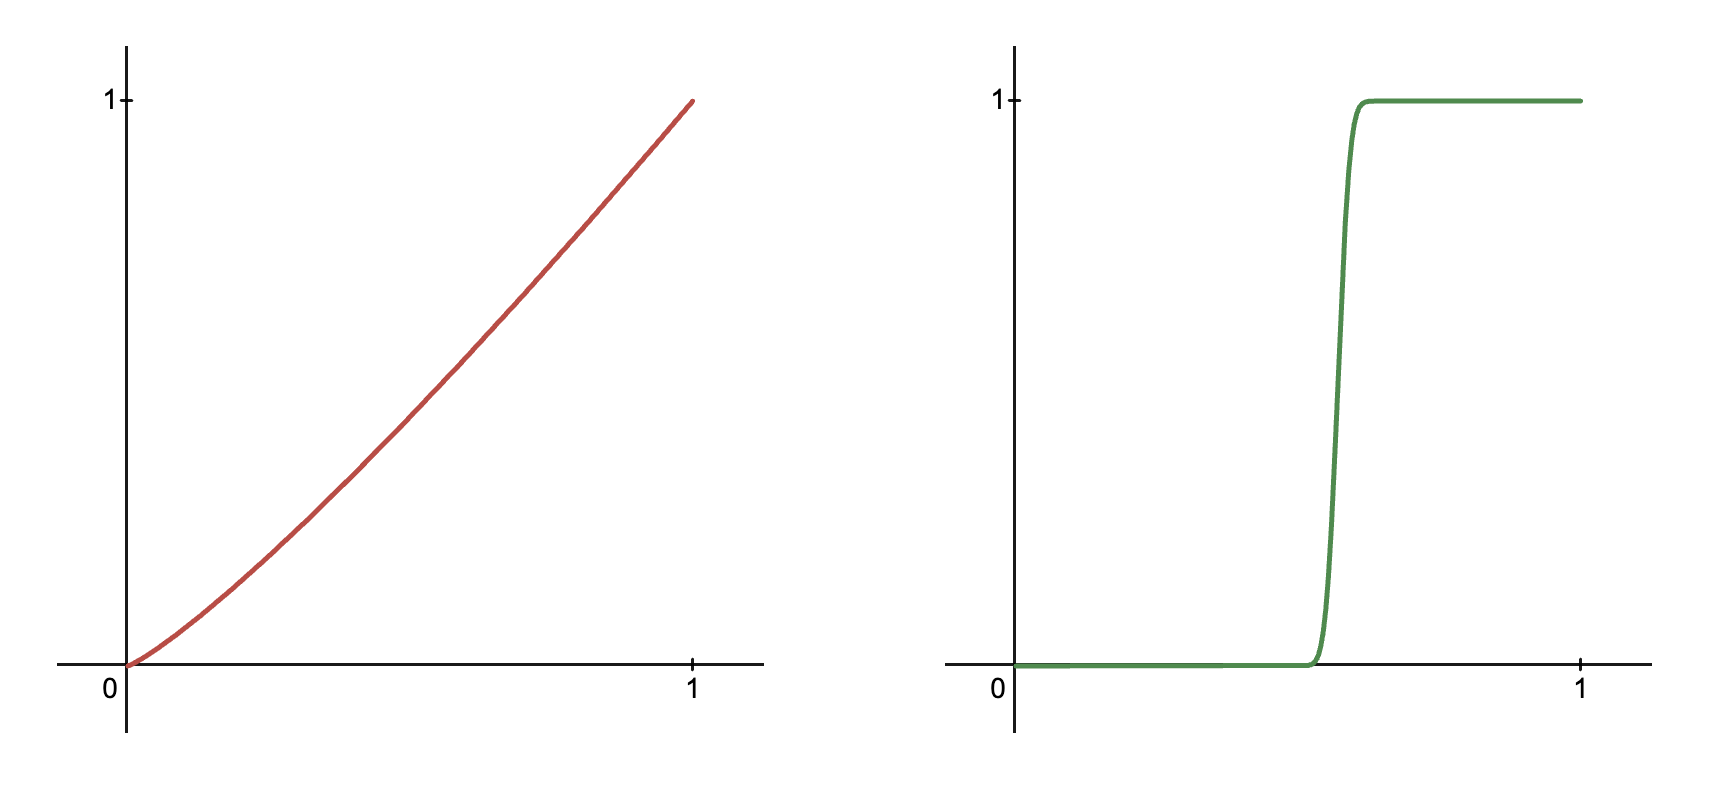
\includegraphics[width=0.6\textwidth]{figures/phase-transition.png}
\end{center}

In fact, it increases as in the phase transition graph on the right!

This demonstrates a \textit{threshold} effect, where the probablity increases very rapidly from 0 to 1 around some threshold value of $p$. Why does this happen, and how can we find the threshold value?

\begin{remark}[Probability Recap]
    Recall that for a discrete random variable $X$ taking values in $\N_0$, to show $\P[X = 0]$ is large, it is sufficient to show that $\mu = \E[X]$ is small. Indeed, for all $t > 0$, we have $\mu \geq t \P[X \geq t]$, so $\P[X \geq t] \leq \mu / t$ (Markov's inequality), so $\P[X = 0] \geq 1 - \mu$.
    
    The converse is unfortunately false: for any $\P[X = 0] < 1$, $\mu$ can be arbitrarily large. Indeed, to show that $\P[X = 0]$ is small, we need to show that $\sigma^2/\mu^2$ is small, since
    \[
	\sigma^2 = \E[(X - \mu)^2] = \E[X^2] - \E[X]^2 \implies \P((X - \mu)^2 \geq t) \leq \sigma^2/t^2 \text{ for all $t > 0$}.
	\]
	This gives us $\P[X = 0] \leq \sigma^2/\mu^2$ as desired. If $X$ counts the number of events $A$ that occur, meaning $\mu = \sum_A \P(A)$, then the variance is
	\[
	\sigma^2 = \E[X^2] - \E[X]^2 = \sum_{A,B}\P[A]\P[B] - \sum_{A,B} \P[A \cap B] = \sum_{A,B} \P[A] \cdot (\P[B \mid A] - \P[B]).
	\]
\end{remark}

This lets us write down the behaviour of the threshold function.

\begin{theorem}[Phase Transition]
    Given constant $\lambda$, let $G \in \calG(n, p)$, where $p = \lambda \ln(n) / n$. Then if $\lambda < 1$, $G$ almost surely has an isolated vertex, and if $\lambda > 1$ then $G$ almost surely does not have an isolated vertex.
\end{theorem}

\begin{prf}
    Let $X$ be the random variable counting the number of isolated vertices, with $I_v$ being the indicator variable for a vertex $v$ being isolated. Then
    \[
	\mu = \E[X] = \sum_{v \in V} I_v = n(1-p)^{n-1} = \frac{n}{1-p} (1-p)^n.
	\]
	For $\lambda > 1$, we have:
	\[
	\mu \leq \frac{n}{1-p} e^{-pn} = \frac{n}{1-p} e^{-\lambda \ln n} = \frac{n^{1-\lambda}}{1-p} \to 0 \text{ as $n \to \infty$.}
	\]
	This means that $\P[X = 0] \to 1$ as $n \to \infty$, which means $X = 0$ almost surely.
	
	Conversely, for $\lambda < 1$, for any $\eps>0$ and sufficiently small $p$ we have:
	\[
	1 - p \geq e^{-(1 + \eps)p} \implies \mu \geq \frac{n}{1-p} e^{-(1+\eps)pn} = \frac{n}{1-p} e^{-(1+\eps)\lambda \ln n} = \frac{n^{1 - (1+\eps)\lambda}}{1-p}.
	\]
	If we choose $\eps < \lambda^{-1} - 1$ , then $\mu \to \infty$ as $n \to \infty$. Also,
	\[
	\sigma^2 = \sum_{u,v \in V} \P[I_u = 1] \left( \P[I_v = 1 \mid I_u = 1] \P[I_v = 1] \right)
	\]
	This is equal to a series of $n$ terms with $u = v$, and $n(n-1)$ terms with $u \neq v$, so we have
	\begin{align*}
    \sigma^2 &= n(1-p)^{n-1} \left( 1 - (1-p)^{n-1} \right) + n(n-1)(1-p)^{n-1} \left( (1-p)^{n-2} - (1-p)^{n-1} \right) \\
    &\leq \mu + n(n-1) (1-p)^{n-1} p (1-p)^{n-2}  \leq \mu + p\mu^2/(1-p)
	\end{align*}
	Therefore $\sigma^2/\mu^2 \leq 1/\mu + p/(1-p) \to 0$ as $n \to \infty$, and so $X \neq 0$ almost surely.
\end{prf}

So $p = \ln n / n$ is a threshold value for the property of having an isolated vertex, since for all $\lambda < 1$, we have $p = \lambda \ln n / n$ implying that the probability of having an isolated vertex is zero, and for all $\lambda > 1$, the probability is one.

A different kind of threshold effect comes from considering the clique number $\mathrm{CL}(G)$. Here, we fix $p$ and increase $n$ to consider graphs in $\calG (n, p)$. We might guess that the distribution follows a roughly bell-shaped distribution, but in fact there is a very narrow spike.

\begin{proposition}[Random Clique Numbers]
    Let $0 < p < 1$ be fixed, and let $d$ be a real number such that
    \[
	\binom n d \times p^{\binom d 2} = 1.
	\]
	Then almost surely, $G \in \calG (n, p)$ has clique number $\ceil{d}$, $\floor{d}$, or $\floor{d} - 1$.
\end{proposition}

\begin{prf}
    Fix $k$ and let the random variable $X$ be the number of copies of $K_k$ in $G$. Note that
    \[
	\mu = \E[X] = \binom n k \times p^{\binom k 2} \text{, much like our expression involving $d$.}
	\]
	Note that $X = \sum_\alpha I(\alpha)$, where $I(\alpha)$ is a set of indicator variables indicating that $G[\alpha]$ is complete. Here, $\alpha$ runs over the $k$-sets of $\set{1 \dots n}$.
	
	If $k \geq d+1$, then we see that $\mu \to 0$ as $n \to \infty$, so $X = 0$ almost surely.
	
	If $k \leq d-1$, then we see that $\mu \to \infty$ as $n \to \infty$. Also,
	\[
	V = \binom n k \times p^{\binom k 2} \times \sum_{s=2}^k \binom k s \binom{n-k}{k-s} \left( p^{\binom k 2 - \binom s 2} - p^{\binom k 2} \right)
	\]
	Actually, there is some $d$ such that $\mathrm{CL}(G)$ is $d$ or $d+1$ almost surely. In the sum, the first term is equal to
	\[
	\binom k 2 \binom{n-k}{k-2} p^{\binom k 2} \left( \frac{1}{p} - 1 \right) \leq \binom k 2 \binom{n-k}{k-2} p^{\binom k 2 - 1}
	\]
	while the last term is at most 1. We can also check that these terms dominate the sum, so $V / \mu^2 \to 0$ as $n \to \infty$. This means that $X \neq 0$ almost surely, as we desired. 
\end{prf}

% ================================================================== %

\pagebreak
\section{Algebraic Methods}
\subsection{Moore Graphs}

Previously, Definition \ref{distance-definition} specified the \textit{distance} function as a metric on a graph, given by the minimum path length between two vertices. Further, we also mentioned the \textit{diameter} of a graph, which is defined to be
\[
\mathrm{diam}(G) = \max \set{d(x, y) : x, y \in V}.
\]
\begin{corollary}
	$G$ has diameter 1 if and only if $G$ is complete (and has at least two vertices).
\end{corollary}

\begin{corollary}
	The diameter of $G$ is finite if and only if $G$ is connected.
\end{corollary}

The motivating question for this section is ``how many vertices can a graph with maximum degree $\Delta$ have, given that the diameter is at most 2?"

We first try expanding from a vertex $x$. $V(G) \subs \set x \cup \Gamma(x) \cup \Gamma(\Gamma(x))$. Thus
\[
n = \abs G \leq 1 + \Delta + \Delta(\Delta - 1) = 1+\Delta^2
\]
is an upper bound. Is it possible to attain this bound? Observe that any graph which does so must be regular, as $x$ was an arbitrary vertex which provides bound $1 + d(x)^2$.

\begin{definition}[Moore Graph]
    A $k$-regular graph of diameter 2 on $1+k^2$ vertices is called a \textit{Moore graph}. Equivalently, a $k$-regular graph is a Moore graph if and only if every distinct pair of vertices $x \neq y$ has a unique path between them of length at most 2.
\end{definition}

Moore graphs cannot contain copies of $C_3$ or $C_4$, otherwise there would be multiple paths of length at most 2. This means that the girth of any Moore graph $G$ is at least 5.

For $k = 2$, we have $\abs G = 2^2 + 1 = 5$. The only graph of order 5 with girth at least 5 is $C_5$.

For $k = 3$, we have $\abs G = 3^2 + 1 = 10$. In fact, the Moore graph with $k=3$ is the Petersen graph!

\ \ctikzfig{small-moore-graphs} \

We might conjecture that there are infinitely many such graphs, with one for each $k$. However, there are in fact fewer than five!

The only Moore graphs are with $k = 2$, $k = 3$, $k = 7$, and possibly $k = 57$. We will devote the rest of the section to proving this.

% ================================================================== %

\subsection{Adjacency Matrices}

\begin{definition}[Adjacency Matrix]
    Let $G = (V, E)$ be a graph on $V = \set{1 \dots n}$. The \textit{adjacency matrix} of $G$ is the $n \times n$ matrix $A$ with entries
    \[
	a_{ij} = \begin{cases}
		1 & ij \in E \\
		0 & \otherwise
	\end{cases}
	\]
	This is always a real and symmetric (thus diagonalisable) matrix with zero trace.
\end{definition}

\begin{example}[Adjacency Matrix]
    We can draw an adjacency matrix for an arbitrary graph using this relation:
    
    \ctikzfig{adjacency-matrix-definition}
\end{example}

The adjacency matrix $A$ encodes all the information inherent in $G$, so theoretically every property of $G$ is recoverable through $A$. In fact, we can use the matrix directly to show some results.

Recall the idea of a walk from Definition \ref{walk-definition}: a walk of length $r$ from $u_0$ to $u_r$ is a sequence $u_0u_1\dots u_r$ of $r+1$ (not necessarily distinct) vertices, where each $u_{i-1}$ is connected to $u_i$.

Now consider the matrix $A^2$ = $A \times A$. We have
\[
(A^2)_{ij} = \sum_{k=1}^n A_{ik} \cdot A_{kj} = \begin{cases}
	\text{the number of common neighbours of $i$ and $j$} \\
	\text{the number of walks of length 2 from $i$ to $j$}
\end{cases}
\]
which is equal to $\abs{\Gamma(i) \cap \Gamma(j)}$.

In general, $(A^r)_{ij}$ is the number of walks of length $r$ from $i$ to $j$.

There is a linear map $\R^n \to \R^n$ which maps $x \mapsto Ax$, where
\[
(A_\lambda)_i = \sum_{j = 1}^n A_{ij} \cdot x_j
\]
Given a graph with adjacency matrix $A$ with each vertex labelled with a number $x_i$, applying $A$ to the vector $x$ gives $Ax$, where each entry is the sum of the labels of each neighbour.

Since $A$ is real and symmetric, it is diagonalisable, and so there is a basis of orthonormal eigenvectors $e_1 \dots e_n$ with corresponding eigenvalues $\lambda_1 \geq \lambda_2 \geq \dots \geq \lambda_n$. (We can take orthonormality and descending eigenvalues without loss of generality by reordering and scaling.)

Write $\lambda_\text{max} = \lambda_1$ and $\lambda_\text{min} = \lambda_n$. We have $\sum \lambda_i = \tr A = 0$. Unless $G = E_n$, this means $\lambda_\text{min} < 0$ and $\lambda_\text{max} > 0$.

Suppose that $e_1 \dots e_n$ is an orthonormal basis of eigenvectors. Take $x \in \R^n$ and write $x = \sum c_i e_i$ for $c_i \in \R$. with $\abs{x} = \sum c_i^2 = 1$. Then $Ax = \sum c_i \lambda_i e_i$, and so $\angled{Ax, x} = (Ax) \cdot x = \sum \lambda_i c_i^2$. Therefore
\[
\lambda_\text{max} = \max_{\abs{x} = 1} \angled{Ax, x} \quad \text{and} \quad \lambda_\text{min} = \min_{\abs{x} = 1} \angled{Ax, x}
\]

\begin{proposition}[Eigenvalue Bounds]
    Suppose $G$ is a connected graph with adjacency matrix $A$.
    \begin{enumerate}
	    \item If $\lambda$ is an eigenvalue of $G$, then $\abs{\lambda} \leq \Delta(G)$.
	    \item $\Delta$ is an eigenvalue if and only if $G$ is regular, in which case its eigenvector is $(1, 1, \dots, 1)$ and its multiplicity is 1.
	    \item $-\Delta$ is an eigenvalue if and only if $G$ is regular and bipartite. Its multiplicity is then 1.
	    \item $\lambda_\text{max} \geq \delta(G)$.
	\end{enumerate}
\end{proposition}

\begin{prf}
    Consider the adjacency matrix $A$.
    \begin{enumerate}
	    \item Choose the eigenvector $x = (x_1 \dots x_n) \neq 0$ with eigenvalue $\lambda$. Let $i$ be such that $\abs{x_i}$ is maximal. Without loss of generality, take $x_i = 1$, so for all $j$ we have $\abs{x_j} \leq 1$. Then
		\[
			\abs{\lambda} = \abs{\lambda x_i} = \abs{(Ax)_i} = \abs{\sum_{j=1}^n A_{ij}x_j} = \abs{\sum_{j \in \Gamma(i)} x_j} \leq \sum_{j \in \Gamma(i)} \abs{x_j} = d(i) \leq \Delta(G)
		\]
		\item If $G$ is $\Delta$-regular, then clearly $x = (1,1, \dots 1)$ is an eigenvector with eigenvalue $\Delta$. Conversely, taking $\lambda = \Delta$ in the first point gives $\Delta = (Ax)_i = \sum x_j$ for the neighbours $j$ of $i$. Hence $d(i) = \Delta$, and this is true for all $i$.
		\item Taking $x = 1$ on $X$ and $-1$ on $Y$ where $X \cup Y$ is our bipartition, then $Ax = -\Delta x$. Conversely, if $-\Delta$ is an eigenvalue, then the sum
		\[
			\sum_{j \in \Gamma(i)} x_j = -\Delta \implies d(i) = \Delta \text{ and }x_j = -1 \text{ for every } j \in \Gamma(i).
		\]
		Repeating this gives us $G$ being $\Delta$-regular, and $x_k = \pm 1$ with $x_i x_j = -1$ for all edges (as $G$ is connected). $G$ is then bipartite: we can partition it by the sign of the vertex label.
		\item We must find $x$ with $\abs x = 1$ and $\angled{Ax, x} \geq \delta$. Take $x = (1, 1, \dots 1)$. Then $(Ax)_i \geq \delta$, so $\angled{Ax, x} \geq \delta \angled{x, x} = \delta n$. Thus $\lambda_\text{max} \geq \delta$. 
	\end{enumerate}
	Thus all four results hold.
\end{prf}

By Brooks's Theorem (\ref{brooks-theorem}), we know that $\chi(G) \leq \Delta + 1$. We can strengthen this bound.

\begin{proposition}[Stronger Brooks's Theorem]
    In fact, for every graph $G$ we have $\chi(G) \leq \lambda_\text{max} + 1 \leq \Delta + 1$.
\end{proposition}

\begin{prf}
    The $\abs G = 1$ case is trivial, so assume $\abs G \geq 2$. Choose $v$ with $d(v) = \delta(G)$, and set $G' = G - v$. If we can show that $\lambda_\text{max}(G') \leq \lambda_\text{max}(G)$, then we are done, as we would be able to colour $G'$ in $\lambda_\text{max} + 1$ colours, and now $d(v) = \delta \leq \lambda_\text{max}$, which means we can also colour $v$.
    
    Now let $A$ and $B$ be the adjacency matrices of $G$ and $G'$. $B$ is formed form $A$ by deleting the $v$'th row and column. Without loss of generality, this is the last row and column. So we must show that
    \[
	\max_{x \in \R^{n-1}, \abs{x} = 1} \angled{Bx, x} \leq \max_{x \in \R^{n}, \abs{x} = 1} \angled{Ax, x}
	\]
	But this is simple, as for any $x = (x_1, x_2, \dots x_{n-1}) \in \R^{n-1}$, then $y = (x_1, x_2, \dots x_{n-1}, 0) \in \R^{n}$ satisfies $\abs{y} = \abs{x}$ and $\angled{Bx, x} = \angled{Ax, x}$.
\end{prf}

In fact, with some more work we could show that for any non-empty graph $G$, the chromatic number $\chi(G) \geq 1 - \lambda_{\text{max}} / \lambda_{\text{min}}$. (Note that the smallest eigenvalue is negative.)

% ================================================================== %

\subsection{Strong Regularity}

Recall our notion of regularity from Definition \ref{regular-definition}. This can be thought of as a sort of indifference or symmetry of vertices, whereby every vertex has the same degree. We expand this notion here.

\begin{definition}[Strong Regularity]
    Let $k, b \geq 1$ and $a \geq 0$. We say that a graph is \textit{strongly regular} with parameters $(k, a, b)$ if $G$ is $k$-regular, and any two distinct vertices $x$ and $y$ have:
    \begin{itemize}
    	\item $a$ common neighbours if $x$ and $y$ are adjacent
    	\item $b$ common neighbours if $x$ and $y$ are not adjacent.
    \end{itemize}
\end{definition}

The Petersen graph is strongly regular with parameters $(3, 0, 1)$. $C_4$ has $(2, 0, 2)$ and $C_5$ has $(2, 0, 1)$. Complete graphs $K_n$ are trivially strongly regular (with $b$ undefined) so we usually ignore them.

We see that a strongly regular graph must be connected: any two distinct vertices are either adjacent or have $b \geq 1$ neighbours in common, so there is a path between any two vertices. In fact, this argument shows that the diameter of $G$ is at most 2. 

We can find other bounds. For example, $a \leq k-1$: if each vertex has has $k$ neighbours, it has at most $k-1$ neighbours in common with each of them.

John Conway (of Game of Life fame) posed the well-known ``99 graph problem", which asks for a $(14, 1, 2)$ strongly regular graph on 99 vertices. Strong regularity is a very restrictive property, so this is quite difficult to achieve, and finding such a graph would have implications for other combinatorial problems.

\begin{theorem}[Hoffman-Singleton Theorem]
    Let $G$ be a graph on $n$ vertices which is not the complete graph. Suppose $G$ is strongly regular with parameters $(k, a, b)$.  Then the numbers
    \[
	\frac{1}{2} \left( n - 1 \pm \frac{(n-1)(a-b)+2k}{\sqrt{(b-a)^2 - 4(b-k)}} \right)
	\]
	are integers.
\end{theorem}

\begin{prf}
    Let $\abs G = n$, and let $A$ be the adjacency matrix of $G$. Clearly, $G$ is connected, and since $G$ is $k$-regular, it has an eigenvalue $k$ for the eigenvector $v = (1, \dots, 1)$ of multiplicity 1. Let $\lambda \neq k$ be an eigenvalue with eigenvector $x$. Taking $A^2$ gives the number of walks of length 2, so
    \[
	(A^2)_{ij} = \begin{cases}
		k & i=j \\
		a & ij \in E(G) \\
		b & \otherwise
	\end{cases}
	\]
	Thus we have
	\begin{align*}
    	A^2 &= kI + aA + b(J-I-A) \qquad \where J_{ij} = 1 \\
    	\implies A^2 + &(b-a)A + (b-k) I = bJ
	\end{align*}
	Applying $A$ to $x$, noting that $\angled{x, v} = 0$, so $Jx = 0$. Thus
	\[
	\lambda^2 x = kx + a\lambda x - bx - b \lambda x \implies \lambda^2 + (b-a)\lambda + (b-k) = 0
	\]
	The remaining eigenvalues are therefore given by
	\[
	\lambda, \mu = (1/2) \times (a-b \pm \sqrt{(b-a)^2 - 4(b-k)}).
	\]
	Suppose these have multiplicities $r$ and $s$. As $A$ is diagonalisable, we have $r+s+1=n$. Also, since $\tr(A) = 0$, we have $\lambda r + \mu s + k = 0$. Subtracting our equations gives us
	\[
	(\lambda - \mu) s = \lambda(n-1) + k \qquad \text{and} \qquad \lambda - \mu = \sqrt{(b-a)^2 - 4(b-k)},
	\]
	which finally gives us the multiplicities we desire:
	\[
	s, r = \frac{1}{2} \left( n - 1 \pm \frac{(n-1)(a-b)+2k}{\sqrt{(b-a)^2 - 4(b-k)}} \right).
	\]
	Of course, these must be integers, which completes the proof.
\end{prf}

So the adjacency matrix $A$ really is quite powerful! We can actually prove a much more significant theorem using this result, which we claimed earlier.

\begin{theorem}[At Most Four Moore Graphs]
    Let $G$ be a Moore graph of degree $k$. Then $k \in \set{2, 3, 7, 57}$.
\end{theorem}

\begin{prf}
    Moore graphs are strongly regular with degree $k$ and parameters $(k^2 + 1, 0, 1)$. Thus
\[
\frac{1}{2} \left( k^2 \pm \frac{2k-k^2}{\sqrt{4k-3}} \right) \in \Z
\]
	If $2k - k^2 = 0$, this gives us the $k=2$ case. Otherwise, $4k-3 = t^2$ for some $t \in \N$ with $t \divides (2k-k^2)$. Then we have
	\[
	k = \frac{t^2 + 3}{4} \qquad \text{and} \qquad k^2 - 2k = tr
	\]
	for some $r \in \Z$. This gives
	\[
	\left( \frac{t^2+3}{4} \right)^2 - 2 \left( \frac{t^2+3}{4} \right) = tr \implies t^4 - 2t^2 - 16tr - 15 = 0
	\]
	This means that $t \mid 15$, so $t \in \set{1, 3, 5, 15}$. This gives $k \in \set{1, 3, 7, 57}$, along with the $k=2$ case.
	
	However, $k=1$ has the wrong diameter, so we are left with the four cases $k \in \set{2, 3, 7, 57}$.
\end{prf}

\begin{remark}[Finding All Moore Graphs]
    Can we actually find these graphs?
	\begin{enumerate}
	    \item For $k=2$, we have $C_5$.
	    \item For $k=3$, we have the Petersen graph.
	    \item For $k=7$, we have the Huffman-Singleton graph, which is $7$-regular on $50$ vertices and 175 edges. We construct this using five pentagons $P_0 \dots P_4$ and five pentagrams $Q_0 \dots Q_4$. We then adjoin vertex $t$ in $P_i$ to vertex $t + ij$ in $Q_j$, where indices are taken modulo 5.
	    \item For $k=57$, we seek a $57$-regular graph on 3250 vertices with diameter 2. Such a graph is not yet found, and so it is often called the \textit{missing Moore graph}.
	\end{enumerate}
\end{remark}

\begin{note}
	We know that if the missing Moore graph exists, it cannot be vertex-transitive.
\end{note}

This is because the automorphism group $\mathrm{Aut}(G)$ acts transitively on vertices, so given $v_1$ and $v_2 \in G$ there would necessarily be an automorphism $\sigma$ satisfying $\sigma(v_1) = v_2$. In this case, $\abs{\mathrm{Aut}(G)} \leq 375 < 3250 = \abs{G}$, so there cannot be such an automorphism.

% ================================================================== %

\subsection{Group Theory}

$\mathrm{Aut}(G)$ is the group of permutations of vertices preserving adjacency. Robert Frucht proved in 1939 that every finite group can be represented as the automorphism group of some finite graph. In fact, it was showed 20 years later that \textit{any} group can be represented as the automorphism group of some (now possibly finite) graph, if one assumes the axiom of choice.

\begin{definition}[Vertex Space]
    The \textit{vertex space} $C_0 (G)$ of a graph $G$ is the $\C$-vertex space of all functions $V(G) \to \C$. If $V(G) = \set{v_1 \dots v_n}$, then the dimension of $C_0(G)$ is in fact $n$. Elements of this space are of the form
    \[
	x = \sum_{i=1}^n x_i v_i = \underbrace{(x_i)^n}_{\text{weights}}.
	\]
\end{definition}

Each $\pi \in \mathrm{Aut}(G)$ induces an endomorphism of $C_0(G)$, given by the permutation matrix $P$. But any permutation matrix corresponds to an endomorphism precisely when it commutes: $AP = PA$. This group of matrices is therefore a faithful representation of $\mathrm{Aut}(G)$.

As always, everything comes back to graph theory: the classification of finite simple groups (as in the famous ATLAS of Finite Groups) also relies on graphs!



\end{document}